\documentclass{article}

\title{
	Finding Optimal Diverse Feature Sets\\
	via Alternative Feature Selection
}
\author{
	Jakob Bach~\orcidlink{0000-0003-0301-2798}\\
	\small Karlsruhe Institute of Technology (KIT), Germany\\
	\small \href{mailto:jakob.bach@kit.edu}{jakob.bach@kit.edu}
}
\date{} % don't display a date

\usepackage[style=numeric, backend=bibtex]{biblatex}
\usepackage[ruled,linesnumbered,vlined]{algorithm2e} % pseudo-code
\usepackage{amsmath} % mathematical symbols
\usepackage{amssymb} % mathematical symbols
\usepackage{amsthm} % theorems, definitions etc.
\usepackage{booktabs} % nicely formatted tables (with top, mid, and bottom rule)
\usepackage{graphicx} % plots
\usepackage{orcidlink} % ORCID icon
\usepackage{subcaption} % figures with multiple sub-figures and sub-captions
\usepackage{hyperref} % links and URLs

\addbibresource{references.bib}

\theoremstyle{definition}
\newtheorem{definition}{Definition}

\begin{document}

\maketitle

\begin{abstract}
Feature-selection methods are popular to obtain small, interpretable, yet highly accurate prediction models.
Existing feature-selection methods typically yield only one feature set, which might not be sufficient in some cases.
For example, users might be interested in finding different feature sets with similar prediction quality, offering alternative explanations of the data.
In this article, we introduce and formalize alternative feature selection as an optimization problem.
Next, we show how to integrate various categories of existing feature-selection methods.
Finally, we evaluate alternative feature selection in a study with 30 classification datasets.
In our experiments, we observe a trade-off between the feature-set quality and how alternative the feature sets should be.
\end{abstract}
%
\textbf{Keywords:} feature selection, alternatives, constraints, mixed-integer programming, explainability, interpretability, XAI

\section{Introduction}
\label{sec:afs:introduction}

\paragraph{Motivation}

Feature-selection methods are ubiquitous for a variety of reasons.
By reducing dataset dimensionality, they lower the computational and memory requirements of prediction models.
Next, models might generalize better after removing irrelevant and spurious predictors.
Finally, prediction models might become simpler and more comprehensive~\cite{li2017feature}, improving interpretability.

Traditional feature-selection methods mostly return only one feature set~\cite{borboudakis2021extending}.
These methods optimize a criterion of feature-set quality, e.g., prediction performance.
However, besides the optimal feature set, there might be other, differently composed feature sets with similar quality.
For the user, these alternative feature sets might be interesting for multiple reasons.
First, some originally selected features might be costly to obtain, so the user would prefer cheaper alternatives.
Second, some originally selected features might contain sensitive information that should not be used in predictions.
Third, the user might be interested in explanations for the prediction, rather than just making good predictions.
In such a situation, knowing alternatives allows the formulation of multiple hypotheses and broadens the understanding.

\paragraph{Problem statement}

This article addresses the problem of alternative feature selection, which we informally define as follows:
%
\begin{definition}[Alternative feature selection (informal)]
	Given an original feature set, find a sufficiently different feature set that optimizes feature-set quality.
	\label{def:afs:alternative-feature-selection}
\end{definition}
%
We provide formal definitions in Section~\ref{sec:afs:approach:constraints}.
Ideally, the alternative feature set should have a similar quality as the original one.
However, depending on how different the alternative feature set should be, one might have to compromise on quality.
E.g., if there are only a few highly predictive features and most of them are part of the original feature set, the alternative feature set might have significantly lower prediction quality.
We analyze this effect in our article.
Also, we consider finding multiple alternatives rather than just one.

Two points are essential for alternative feature selection, which we both address in this article.
First, one needs to formalize and quantify what an alternative feature set is.
Second, one needs an approach to find alternative feature sets efficiently.
Ideally, the approach should be general, i.e., cover a broad range of existing feature-selection methods.

\paragraph{Related work}

While finding alternative solutions has already been addressed extensively in the field of clustering~\cite{bailey2014alternative}, there is a lack of such approaches for feature selection.
Only few feature-selection methods target at obtaining multiple, diverse feature sets~\cite{borboudakis2021extending, siddiqi2020genetic}.
In particular, techniques for ensemble feature selection~\cite{saeys2008robust, seijo2017ensemble} and statistically equivalent feature subsets~\cite{lagani2017feature} produce multiple feature sets but not optimal alternatives.
In fields related to feature selection, the goal of obtaining multiple, diverse solutions has been studied as well, e.g., for subspace clustering~\cite{mueller2009relevant}, subspace search~\cite{trittenbach2019dimension}, or explainable-AI techniques~\cite{artelt2022even, kim2016examples, mothilal2020explaining, russell2019efficient} like counterfactuals.
However, these works address different problems than alternative feature selection, as we discuss in Section~\ref{sec:afs:related-work}.

\paragraph{Contributions}

Our contribution is threefold.
First, we formalize alternative feature selection as an optimization problem.
In particular, we define alternatives via constraints on feature sets.
Second, we discuss approaches to solve this optimization problem.
To that end, we describe how to integrate different categories of feature-selection methods in the objective function.
Third, we evaluate alternative feature selection with comprehensive experiments.
We use 30 classification dataset from the Penn Machine Learning Benchmarks (PMLB)~\cite{olson2017pmlb, romano2021pmlb} and four feature-selection methods.
We focus on the question if one can find alternative feature sets with similar feature-set quality as the original ones.

Our definition of alternatives is orthogonal to existing feature-selection methods, i.e., not tailored towards specific techniques.
Further, this formulation allows integrating other constraints on feature sets, e.g., based on domain knowledge~\cite{bach2022empirical, groves2015toward}.
Finally, we only require users to set two parameters, i.e., the number of alternatives and a dissimilarity threshold for feature sets being alternative.
In fact, one can see existence of these parameters positively, as they allow users to control the search for alternatives according to their needs.

\paragraph{Results}

Depending on the dataset and the parameters for searching alternatives, we could find alternative feature sets with similar quality as the original ones.
This outcome encourages using alternative feature sets as a tool for alternative explanations of predictions.
As expected, feature-set quality tends to decrease with the number of alternatives.
The exact decrease depends on how the feature-set quality is distributed in the dataset.
Further, we observed that the quality of alternative feature sets significantly depends on the dissimilarity threshold for being alternative.
Thereby, this threshold allows the user to exercise use-case-specific control on the trade-off between feature sets being alternative and having high feature-set quality.
We publish our code\footnote{\url{https://github.com/Jakob-Bach/Alternative-Feature-Selection}} and our experimental data\footnote{\url{https://www.dropbox.com/sh/3bmeoihgozmvfg3/AAD9AcRddqRVlu7tps6FxIKIa?dl=0}} online. % TODO

\paragraph{Outline}

Section~\ref{sec:afs:fundamentals} explains fundamentals of feature selection.
Section~\ref{sec:afs:approach} defines the problem of alternative feature selection and discusses solution approaches.
Section~\ref{sec:afs:related-work} reviews related work.
Section~\ref{sec:afs:experimental-design} describes our experimental design and Section~\ref{sec:afs:evaluation} presents the experimental results.
Section~\ref{sec:afs:conclusion} concludes.

\section{Fundamentals}
\label{sec:afs:fundamentals}

In this section, we introduce basic notation and review different methods to measure the quality of feature sets.

\subsection{Notation}
\label{sec:afs:fundamentals:notation}

Let $X \in \mathbb{R}^{m \times n}$ be a dataset represented as a matrix.
Each row is a data object, and each column is a feature.
Let $F = \{f_1, \dots, f_n\}$ denote the set of feature names.
We assume categorical features have already been made numeric, e.g., via one-hot encoding.
Let $X_{\cdot{}j} \in \mathbb{R}^m$ denote the vector representation of the $j$-th feature.
Further, let $y \in \mathbb{R}^m$ represent the prediction target.
The actual domain of the target might also be smaller, e.g., $\{0,1\}$ for binary classification.

With feature selection, one makes a binary decision $s_j \in \{0,1\}$ for each feature, i.e., either selects it or not.
The vector $s \in \{0,1\}^n$ combines all these selection decisions.
The selected feature set is $F_s = \{f_j \mid s_j=1\}$.
Let the function $Q(s,X,y)$ return the quality of such a feature set.
Without loss of generality, we assume this function should be maximized.

\subsection{Measuring Feature (Set) Quality}
\label{sec:afs:fundamentals:quality}

There are different ways to evaluate feature-set quality $Q(s,X,y)$.
Note that we only give a short overview here; see~\cite{chandrashekar2014survey,li2017feature} for comprehensive surveys of feature selection.
A traditional categorization of feature-selection methods distinguishes between filter, wrapper, and embedded methods~\cite{guyon2003introduction}.

\paragraph{Filter methods}

Filter methods evaluate feature sets without training a prediction model.
Univariate filters assess each feature independently, often assigning a score to each feature, while multivariate filters evaluate feature sets.
Examples for univariate filters are the absolute Pearson correlation or the mutual information between a feature and the prediction target.
Such methods ignore potential interaction between features, e.g., if they are redundant to each other.
In contrast, multivariate methods often combine a measure of feature relevance with a measure of feature redundancy.
Examples for such methods include CFS~\cite{hall1999correlation, hall2000correlation}, FCBF~\cite{yu2003feature}, and mRMR~\cite{peng2005feature}.
Another popular filter method is Relief~\cite{kira1992feature, robnik1997adaptation}, which assigns quality to individual features rather than feature sets but still uses other features indirectly in nearest-neighbor computations.

\paragraph{Wrapper methods}

Wrapper methods~\cite{kohavi1997wrappers} employ a generic search strategy over feature sets, e.g., genetic algorithms.
Feature-set quality is a black-box function:
Wrappers evaluate candidate feature sets from the search by training prediction models with them and measuring prediction quality.

\paragraph{Embedded methods}

Embedded methods train prediction models with built-in feature selection, e.g., decision trees~\cite{breiman1984classification} or random forests~\cite{breiman2001random}.
Thus, the criterion for feature-set quality is model-specific.
For example, tree-based models often use information gain or the Gini index to select features during training.

\paragraph{Post-hoc feature-importance methods}

Apart from traditional feature selection, there are various methods that assess feature importance after training a model.
These methods range range from local explanation methods like LIME~\cite{ribeiro2016should} or SHAP~\cite{lundberg2017unified} to global importance methods like permutation importance~\cite{breiman2001random} or SAGE~\cite{covert2020understanding}.
In particular, assessing feature importance plays a crucial role in the emerging field of ML interpretability~\cite{carvalho2019machine, molnar2020interpretable}.

\section{Alternative Feature Selection}
\label{sec:afs:approach}

In this section, we present the problem and approaches for alternative feature selection.
First, we define the structure of the optimization problem, i.e., objective and constraints.
Second, we formalize the notion of alternatives via constraints.
Third, we discuss different objective functions, corresponding to different feature-set quality measures from Section~\ref{sec:afs:fundamentals:quality}.
In particular, we describe how to solve the resulting optimization problem.

\subsection{Optimization Problem}
\label{sec:afs:approach:problem}

In alternative feature selection, there are two goals.
First, the quality of an alternative feature set should be high.
Second, an alternative feature set should differ from one or more existing feature set(s).
There are different ways to combine these two goals in an optimization problem:

First, one can consider both goals as objectives, obtaining an unconstrained multi-objective problem.
Second, one can treat feature-set quality as objective and enforce alternatives with constraints.
Third, one can consider being alternative as objective and constrain feature-set quality, e.g., with a lower bound.
Fourth, one can define constraints for both, feature-set quality and being alternative, searching for feasible solutions instead of optimizing.
Depending on the use case, any of these four formulations might be appropriate.

Following the informal Definition~\ref{def:afs:alternative-feature-selection} from the introduction, we stick to the second formulation, i.e., optimizing feature-set quality subject to being alternative.
This formulation has the advantage of keeping the original objective function of feature selection.
Consequently, one does not need to specify a range or a threshold on feature-set quality.
Instead, the user can control how alternative the new feature set should be.
This yields the following optimization problem:
%
\begin{equation}
	\begin{aligned}
		\max_s &\quad Q(s,X,y) \\
		\text{subject to:} &\quad F_s~\text{being alternative}
	\end{aligned}
	\label{eq:afs:afs-general}
\end{equation}
%
We discuss different constraints for \emph{being alternative} and different objective functions $Q(s,X,y)$ in the following.
Additionally, many feature-selection methods also limit the feature-set size $|F_s|$ to a user-defined value~$k \in \mathbb{N}$, as we do in our experiments as well.
Such a requirement on feature-set cardinality adds a further, simple constraint to the optimization problem.

\subsection{Constraints -- Defining Alternatives}
\label{sec:afs:approach:constraints}

In this section, we formalize alternative feature sets.
First, we discuss the base case where an individual feature set is an alternative to another one.
Second, we extend this notion to multiple alternatives, considering sequential as well as simultaneous search procedures.

Our notion of alternatives is independent of the feature-selection method.
We provide two parameters, i.e., a dissimilarity threshold~$\tau$ and the number of alternatives~$a$, which both allow users to control the search for alternatives.

\subsubsection{Single Alternative}
\label{sec:afs:approach:constraints:single}

We consider a feature set to be an alternative to another feature set if it differs sufficiently.
Mathematically, we express this with a set-dissimilarity measure~\cite{choi2010survey, egghe2009new}.
These measures typically assess how strongly two sets overlap and set this in relation to the size of the sets.
For example, a simple and well-known set-dissimilarity measure is the Jaccard distance.
Given two feature sets $F'$, $F''$, the Jaccard distance is defined as follows:
%
\begin{equation}
	d_{\text{Jacc}}(F',F'') = 1 - \frac{|F' \cap F''|}{|F' \cup F''|} = 1 - \frac{|F' \cap F''|}{|F'| + |F''| - |F' \cap F''|}
	\label{eq:afs:jaccard}
\end{equation}
%
Another possible dissimilarity measure follows from the Dice coefficient:
%
\begin{equation}
	d_{\text{Dice}}(F',F'') = 1 - \frac{2 \cdot |F' \cap F''|}{|F'| + |F''|}
	\label{eq:afs:dice}
\end{equation}
%
We leverage such a set-dissimilarity measure for the following definition:
%
\begin{definition}[Single alternative]
	A feature set $F''$ is an alternative to a feature set $F'$ (and vice versa) for a dissimilarity threshold $\tau \in \mathbb{R}_{\geq 0}$ if $d(F',F'') \geq \tau$.
	\label{def:afs:single-alternative}
\end{definition}
%
The threshold~$\tau$ controls how alternative the new feature set should be and depends on the dataset as well as the preferences of the user.
In particular, requiring the new feature set to differ strongly from the existing one might cause a significant drop in feature-set quality.
Some datasets might contain many features of similar utility, thereby enabling many alternatives of similar quality, while predictions on other datasets might depend on a few key features.
Only users can decide which drop in feature-set quality is acceptable for them as a trade-off for obtaining an alternative feature set.
Thus, we leave $\tau$ as a parameter.
In fact, it is the only parameter for our definition of single alternatives, unless one wants to vary the dissimilarity measure for feature sets as well.
In case the set-dissimilarity measure $d(\cdot)$ is normalized to $[0,1]$, like the Dice dissimilarity or Jaccard distance, the interpretation of $\tau$ is user-friendly:
Setting $\tau=0$ allows the alternative feature set to be identical to the original one, while $\tau=1$ requires the two feature sets to have no overlap.

If the choice of $\tau$ is unclear a priori, users can try out different values and compare results.
One potential approach is a binary search:
Start with the mid-range value of $\tau=0$, i.e., 0.5 for $\tau \in [0,1]$.
If the quality of the resulting alternative is too low, decrease $\tau$ to 0.25, i.e., allow more similarity.
If the quality of the resulting alternative is acceptably high, increase $\tau$ to 0.75, i.e., check a more dissimilar feature set.
Continue this procedure till an alternative with an acceptable quality-dissimilarity trade-off is found.

If the feature-set sizes $|F'|$ and $|F''|$ are known, a threshold $\tau$ corresponds to a particular maximum number of overlapping features $|F' \cap F''|$.
This follows from re-arranging Equation~\ref{eq:afs:jaccard} and Equation~\ref{eq:afs:dice} in combination with Definition~\ref{def:afs:single-alternative}:
%
\begin{equation}
	\begin{aligned}
		d_{\text{Jacc}}(F',F'') = 1 - \frac{|F' \cap F''|}{|F'| + |F''| - |F' \cap F''|} &\geq \tau \\
		\Leftrightarrow |F' \cap F''| &\leq \frac{1 - \tau}{2 - \tau} \cdot (|F'| + |F''|)
		\end{aligned}
	\label{eq:afs:jaccard-rearranged}
\end{equation}
%
The latter formulation also avoids having the feature-set sizes, and thereby the decision variables for feature selection, in a quotient.
However, the effect of $\tau$ on the maximum overlap size $|F' \cap F''|$ is non-linear for the Jaccard distance in Equation~\ref{eq:afs:jaccard-rearranged}.
Thus, we use the Dice dissimilarity in this article, where the effect of $\tau$ on the maximum overlap size $|F' \cap F''|$ is linear:
%
\begin{equation}
	\begin{aligned}
		d_{\text{Dice}}(F',F'') = 1 - \frac{2 \cdot |F' \cap F''|}{|F'| + |F''|} &\geq \tau \\
		\Leftrightarrow |F' \cap F''| &\leq \frac{1 - \tau}{2} \cdot (|F'| + |F''|)
	\end{aligned}
	\label{eq:afs:dice-rearranged}
\end{equation}
%
If $|F'| = |F''|$, as in our experiments, the measure becomes identical to several other dissimilarity measures~\cite{egghe2009new}.
Further, $\tau$ then directly controls which fraction of features in one set needs to differ from the other set, and vice versa:
%
\begin{equation}
	\begin{aligned}
		\text{If}~|F'| = |F''|: \quad d_{\text{Dice}}(F',F'') &\geq \tau \\
		\Leftrightarrow |F' \cap F''| &\leq (1 - \tau) \cdot |F'| = (1 - \tau) \cdot |F''|
	\end{aligned}
	\label{eq:afs:dice-rearranged-equal-size}
\end{equation}
%
Thus, if users are uncertain how to choose $\tau$ and $|F''|$ is reasonably small, they can try out all values of $\tau \in \{i / |F''|\}$ with $i \in \{0, 1, \dots, |F''|\}$.
Put differently, $|F''| + 1$ values of $\tau$ cover all potential overlap sizes of the two feature sets.

Up to now, we have used feature sets instead of the binary feature-selection vector $s$.
However, expressing the feature-set sizes in terms of $s$ is straightforward:
%
\begin{equation}
	\begin{aligned}
		|F_s| =& \sum_{j=1}^n s_j \\
		|F_{s'} \cap F_{s''}| =& \sum_{j=1}^n s'_j \cdot s''_j
	\end{aligned}
	\label{eq:afs:feature-set-size}
\end{equation}
%
The expression from Equation~\ref{eq:afs:feature-set-size} also helps to formulate a constraint for limiting the new feature set's size to a user-defined value~$k \in \mathbb{N}$.
Further, combining Equation~\ref{eq:afs:jaccard-rearranged},~\ref{eq:afs:dice-rearranged},~or~\ref{eq:afs:dice-rearranged-equal-size} with Equation~\ref{eq:afs:feature-set-size} yields an inequality only involving sums and products of the binary decision variables and constant values.
In fact, one can replace the product $s'_j \cdot s''_j$, which is non-linear, with linear constraints by introducing an auxiliary variable $t_j$~\cite{mosek2022modeling}:
%
\begin{equation}
	\begin{aligned}
		t_j \leq& s'_j \\
		t_j \leq& s''_j \\
		1 + t_j \geq& s'_j + s''_j \\
		t_j \in& \{0,1\}
	\end{aligned}
	\label{eq:afs:product-linear}
\end{equation}
%
If there is an existing feature set, i.e., either $s'$ or $s''$ is fixed to particular values, Equation~\ref{eq:afs:feature-set-size} already is linear without Equation~\ref{eq:afs:product-linear} since it only multiplies variables with constants in that case.

Overall, one can express alternative feature sets following Definition~\ref{def:afs:single-alternative} with 0-1 integer linear constraints.
This simple constraint type allows using a broad range of solvers, given a suitable objective function, which we discuss later.
One can also encode such constraints into propositional logic (SAT)~\cite{ulrich2022selecting}.

\subsubsection{Multiple Alternatives}
\label{sec:afs:approach:constraints:multiple}

If the user desires multiple alternative feature sets rather than only one, we can compute these alternatives either sequentially or simultaneously.
The number of alternatives~$a$ is a parameter to be set by the user.
Table~\ref{tab:afs:seq-sim-comparison} compares the sizes of the optimization problems for these two search procedures.
%
\begin{table}[htb]
	\centering
	\renewcommand*{\arraystretch}{1.3}
	\begin{tabular}{lccc}
		\toprule
		& \multicolumn{2}{c}{Sequential search} & Simultaneous search \\
		\cmidrule(r){2-3}
		& Alternative $i$ & Summed & \\
		\midrule
		Decision variables~$s$ & $n$ & $ (a+1) \cdot n$ & $(a+1) \cdot n$ \\
		Linearization variables~$t$ & $0$ & $0$ & $\frac{a \cdot (a+1) \cdot n}{2}$ \\
		Alternative constraints & $i$ & $\frac{a \cdot (a+1)}{2}$ & $\frac{a \cdot (a+1)}{2}$ \\
		Linearization constraints & $0$ & $0$ & $\frac{3 \cdot a \cdot (a+1) \cdot n}{2}$ \\
		\bottomrule
	\end{tabular}
	\caption{Size of the optimization problems for $a$ alternatives ($a + 1$~feature sets overall, including the original one) and $n$ features.}
	\label{tab:afs:seq-sim-comparison}
\end{table}
%
\paragraph{Sequential alternatives}

In the sequential case, the user gets several alternatives iteratively, with one alternative feature set per iteration.
We constrain this new feature set to be an alternative to all previously found feature sets:
%
\begin{definition}[Sequential alternative]
	A feature set $F''$ is an alternative to a set of feature sets $\mathbb{F}$ (and vice versa) for a dissimilarity threshold $\tau \in \mathbb{R}_{\geq 0}$ if $\forall F' \in \mathbb{F}: d(F',F'') \geq \tau$.
	\label{def:afs:sequential-alternative}
\end{definition}
%
This definition duplicates the constraint for a single alternative (cf.~Definition~\ref{def:afs:single-alternative}) and instantiates it for multiple existing feature sets.
One could also use a less strict constraint, e.g., based on aggregated dissimilarity, like requiring only the average dissimilarity to all existing feature sets to pass the threshold.
However, definitions like the latter might allow some feature sets to heavily overlap or even be identical if other feature sets are very dissimilar.
Thus, we require pairwise dissimilarity in Definition~\ref{def:afs:sequential-alternative}.
We obtain the following optimization problem, letting $\mathbb{F}$ denote the set of existing feature sets:
%
\begin{equation}
	\begin{aligned}
		\max_s &\quad Q(s,X,y) \\
		\text{subject to:} &\quad \forall F' \in \mathbb{F}: d(F_s,F') \geq \tau
	\end{aligned}
	\label{eq:afs:afs-sequential}
\end{equation}
%
The objective function remains the same as for a single alternative ($|\mathbb{F}| = 1$), i.e., we only optimize the quality of the new feature set~$F_s$.
Thus, the number of variables in the optimization problem is independent of the number of alternatives~$a$.
Instead, we solve the optimization problem repeatedly; each alternative only adds one new constraint to the problem.
As we always compare the new, variable feature set to existing, constant feature sets, we also do not need to introduce interaction variables as in Equation~\ref{eq:afs:product-linear}.
Overall, we expect the runtime of sequential search to scale well with the number of alternatives.
Further runtime gains might be possible if the solver keeps a state between iterations and can warm-start.

However, as the solution space becomes narrower over iterations, feature-set quality can deteriorate with each further alternative.
In particular, multiple alternatives from the same sequential search might differ significantly in their quality.
As a remedy, the user can decide after each iteration if the feature-set quality already is unacceptably low or if another alternative should be found.

\paragraph{Simultaneous alternatives}

In the simultaneous case, we directly obtain multiple alternatives.
The user needs to decide on the number of feature sets $\mathbb{F}$ beforehand.
We formulate pairwise dissimilarity constraints:
%
\begin{definition}[Simultaneous alternatives]
	A set of feature sets $\mathbb{F}$ contains simultaneous alternatives for a dissimilarity threshold $\tau \in \mathbb{R}_{\geq 0}$ if $\forall F' \in \mathbb{F}, F'' \in \mathbb{F}, F' \neq F'': d(F',F'') \geq \tau$.
	\label{def:afs:simultaneous-alternative}
\end{definition}
%
This definition leads to the following optimization problem, assuming we want to obtain $a$ alternative feature sets besides an `original' feature set (which can be any of the solutions since there is no order of feature sets).
%
\begin{equation}
	\begin{aligned}
		\max_{s^{(0)}, \dots, s^{(a)}} &\quad \sum_{i=0}^a Q(s^{(i)},X,y) \\
		\text{subject to:} &\quad \forall i_1 \in \{0, \dots, a\}~\forall i_2 \in \{0, \dots, i_1-1\} : d(F_{s^{(i_1)}},F_{s^{(i_2)}}) \geq \tau
	\end{aligned}
	\label{eq:afs:afs-simultaneous}
\end{equation}
%
In contrast to the sequential case, we need to introduce further decision variables and modify the objective function here, as we optimize multiple feature sets at once.
In Equation~\ref{eq:afs:afs-simultaneous} and our experiments, we consider the summed quality of all feature sets as objective.
Appendix~\ref{sec:afs:appendix:min-quality-objective} presents another objective, which actively balances the quality of all feature sets.
Runtime-wise, we expect simultaneous search to scale worse with the number of alternatives than sequential search, as we need to tackle one large optimization problem instead of multiple smaller ones.
In particular, the number of decision variables increases linearly with the number of alternatives~$a$ and the number of constraints even grows quadratically.
Also, for each feature and each pair of alternatives, we need to introduce an interaction variable as in Equation~\ref{eq:afs:product-linear} if we want to obtain a linear problem.

In contrast to the greedy procedure of sequential search, simultaneous search optimizes alternatives globally.
Thus, the simultaneous procedure should yield same or higher average feature-set quality for the same number of alternatives.
Also, the quality can be more evenly distributed over the alternatives, as opposed to the dropping quality over the course of the sequential procedure.
However, increasing the number of alternatives still has a negative effect on the average feature-set quality.
Further, opposed to the sequential procedure, there are no intermediate steps where the user could interrupt the search.

\subsection{Objective Functions -- Finding Alternatives}
\label{sec:afs:approach:objectives}

In this section, we present approaches for finding alternative feature sets.
We discuss how to solve the optimization problem from Section~\ref{sec:afs:approach:problem} for the different categories of feature-set quality measures from Section~\ref{sec:afs:fundamentals:quality}.
In particular, we categorize solution approaches as white-box optimization, black-box optimization, and embedding alternatives.

\subsubsection{White-Box Optimization}
\label{sec:afs:approach:objectives:white-box}

If the feature-set quality function~$Q(s,X,y)$ is sufficiently simple, one can tackle alternative feature selection with a suitable white-box solver.
In Section~\ref{sec:afs:approach:constraints}, we already showed that our notion of alternative feature sets results in 0-1 integer linear constraints.
In this section, we present white-box optimization objectives for different feature-selection methods.

\paragraph{Univariate filter feature selection}

For univariate filter feature selection, the objective function is linear.
Thus, the optimization problem of alternative feature selection becomes a 0-1 integer linear problem.
Alternatively, one could formulate a weighted partial maximum satisfiability (MaxSAT) problem~\cite{li2021maxsat}.

In particular, univariate filter methods decompose the quality of a feature set into the quality of the individual features:
%
\begin{equation}
	Q_{\text{uni}}(s,X,y) = \sum_{j=1}^{n} q(X_{\cdot{}j},y) \cdot s_j
	\label{eq:afs:univariate-filter}
\end{equation}
%
Here, $q(\cdot)$ typically is a bivariate dependency measure, e.g., mutual information~\cite{kraskov2004estimating} or absolute value of Pearson correlation, to quantify the relationship between a feature and the prediction target.
Appendix~\ref{sec:afs:appendix:complete-optimization-problem} specifies the complete optimization problem including the constraints for alternatives.
Appendix~\ref{sec:afs:appendix:univariate-search-algorithm} presents a procedure to tackle the problem without a solver.

\paragraph{Post-hoc feature importance}

From the technical perspective, one can also insert values of post-hoc feature-importance scores for $q(\cdot)$ in Equation~\ref{eq:afs:univariate-filter}.
For example, one can pre-compute permutation importance~\cite{breiman2001random} or SAGE scores~\cite{covert2020understanding} for each feature.
However, such post-hoc importance scores often evaluate the usefulness of features in the presence of other features.
Thus, the feature-independence assumption underlying Equation~\ref{eq:afs:univariate-filter} does not hold.
In theory, one would have to re-calculate feature importance for each feature set.
However, such a procedure makes a white-box approach infeasible.
In practice, one can still use Equation~\ref{eq:afs:univariate-filter} with importance scores only computed on the full dataset.
One only needs to be aware that such an approach might not represent feature interactions, e.g., feature importances in particular subsets, faithfully.

\paragraph{Multivariate filter feature selection}

Several multivariate filter methods allow for a simple white-box formulation as well, though not necessarily a linear one.
In the following, we describe FCBF~\cite{yu2003feature}, which we use in our experiments.
Appendix~\ref{sec:afs:appendix:multivariate-filter-objectives}~discusses CFS~\cite{hall1999correlation, hall2000correlation}, mRMR~\cite{peng2005feature}, and Relief~\cite{kira1992feature, robnik1997adaptation}.

The Fast Correlation-Based Filter (FCBF)~\cite{yu2003feature} bases on the notion of predominance, expressed by two conditions on selected features:
First, a selected feature's correlation to the prediction target needs to pass a pre-defined threshold.
Second, a selected feature's correlation to the target needs to be higher than each other selected feature's correlation to the given feature.
While the original FCBF algorithm uses a heuristic search to find predominant features, we propose a formulation as a constrained optimization problem:
%
\begin{equation}
	\begin{aligned}
		\max_s &\quad Q_{\text{FCBF}}(s,X,y) = \sum_{j=1}^{n} q(X_{\cdot{}j},y) \cdot s_j \\
		\text{subject to:} &\quad \forall j_1 \in \{2, \dots, n\}, \forall j_2 \in \{1, \dots, j_2 - 1\}: \\
		&\quad \quad\quad \text{If } q(X_{\cdot{}j_1},y) \leq q(X_{\cdot{}j_2}, X_{\cdot{}j_1}): s_{j_1} + s_{j_2} \leq 1
	\end{aligned}
	\label{eq:afs:fcbf}
\end{equation}
%
Our formulation still addresses the two aspects of predominance.
First, we drop the original FCBF's threshold parameter on feature-target correlation and maximize the latter instead, as in the univariate-filter case.
This change can lead to large feature sets, which might containing many low-quality features.
As a countermeasure, one can add a constraint on the feature-set size, as we do in our experiments.
If one still wants to prevent the selection of features with low correlation to the prediction target, one can also filter out these features before optimization.
Second, we keep FCBF's constraints on feature-feature correlation.
In particular, we prevent the simultaneous selection of two features if the correlation between them is at least as high as one of the features' correlation to the target.
As the if-condition in Equation~\ref{eq:afs:fcbf} does not depend on the decision variables~$s$, one can pre-compute whether it holds and add the subsequent linear constraint on~$s$ only if needed.

\subsubsection{Black-Box Optimization}
\label{sec:afs:approach:objectives:black-box}

If feature-set quality has not simple closed-form expression, one needs to treat it as a black-box function when searching for alternative feature sets.
This situation applies to the category of wrapper feature selection.
One can optimize such black-box functions using search heuristics, systematically iterating over candidate feature sets.
However, search heuristics often assume an unconstrained search space.
For example, they might propose a candidate feature set that is not alternative enough.
We see multiple ways to address this challenge:

\paragraph{Enumerating feature sets}

One can relinquish the idea of a search heuristic and just enumerate all feature sets that fulfill the constraints for being alternative.
This most naive idea is iterating over all feature sets and sorting out those not alternative enough.
A bit more focused is using a solver to enumerate all valid alternatives.
While such an approach is technically simple, it might very inefficient, as there can be a huge number of alternative feature sets.

\paragraph{Sampling feature sets}

Instead of considering all possible alternatives, one can also sample a limited number of them.
Again, the naive way is sampling from all feature sets, but removing those samples that are not alternative enough.
If the number of valid alternatives is low relative to the total number of feature sets, this approach might need a lot of samples.
One could also observe the constraints in the sampling procedure, e.g., by using a solver for sampling.
One might abandon the idea of uniform sampling in that case since uniform sampling from a constrained space is a computationally hard problem, believed to be harder than only determining if a valid solution exists or not~\cite{ermon2012uniform}.

\paragraph{Multi-objective optimization}

If one considers alternative feature selection as a multi-objective problem, as mentioned in Section~\ref{sec:afs:approach:problem}, there are no hard constraints anymore.
Given a suitable multi-objective search procedure, the decision on trading off being alternative against feature-set quality might be postponed till after the search.

\paragraph{Adapting search}

One can adapt a search heuristic to consider the constraints for being alternative.
One idea is to prevent the search heuristic from producing feature sets that violate the constraints, or at least making the latter less likely, e.g., be penalizing the objective function accordingly.
Another idea is to `repair' feature sets proposed by the search that are not alternative enough.
For example, one can replace a feature set violating the constraint with the most similar feature set satisfying the constraints.
Such solver-assisted search approaches are common in search procedure for valid configuration in software feature models~\cite{guo2018preserve, henard2015combining, white2010automated}.
One could also apply solver-based repair to randomly sampled feature sets.

As a simple wrapper approach for our experiments, we use a greedy hill-climbing strategy, as displayed in Algorithm~\ref{al:afs:greedy-wrapper}.
Compared to standard hill-climbing~\cite{kohavi1997wrappers}, our search procedure only evaluates feature sets that satisfy the constraints for alternatives.
First, the algorithm uses a solver to find one solution that is alternative enough, given the current constraints.
Thus, it has a valid starting point and can always return a solution, unless there are no valid solutions at all.
Next, it tries `swapping' one feature, i.e., selecting the feature if it was deselected or deselecting it if it was selected.
The algorithm calls the solver again to find a solution~$s'$ containing this change and satisfying the other constraints.
If such a solution~$s'$ exists and its quality~$Q(s',X,y)$ improves the current solution, the algorithm continues from the new solution.
Else, it attempts to swap the next feature.
The algorithm terminates if no swap of a feature leads to an improvement or a fixed amount of iterations $max\_iters$ is reached.
We define the iteration count as the number of calls to the solver, i.e., attempts to generate feature sets, as this step might be costly.
This also is an upper bound on the number of prediction models trained.
However, not all solver calls might yield a valid feature set.

\begin{algorithm}[htb]
	\DontPrintSemicolon
	\KwIn{Dataset $X$, Prediction target $y$, \newline
		Feature-set quality function $Q(\cdot)$, \newline
		Constraints for alternatives $Cons$, \newline
		Maximum number of iterations $max\_iters$}
	\KwOut{Feature-selection decision vector $s$}
	\BlankLine
	$s \leftarrow \text{Solve}(Cons)$ \tcp*{Initial alternative}
	$iters \leftarrow 1$ \tcp*{Number of iterations = solver calls}
	\If(\tcp*[f]{No valid alternative}){$s = \emptyset$}{
		\Return{$\emptyset$}
	}
	$j \leftarrow 1$ \tcp*{Index of feature to be swapped}
	\While{$iters < max\_iters$ \textbf{and} $j \leq |s|$}{
		$s' \leftarrow \text{Solve}(Cons \cup \{\neg s_j\})$ \tcp*{Try swapping one feature}
		$iters \leftarrow iters + 1$\;
		\If(\tcp*[f]{Swap if improved}){$s' \neq \emptyset$ \textbf{and} $Q(s',X,y) > Q(s,X,y)$}{
			$s \leftarrow s'$\;
			$j \leftarrow 1$\;
		}
		\Else(\tcp*[f]{Try next feature}){
			$j \leftarrow j + 1$\;
		}
	}
	\Return{$s$}
	\caption{Constraint-aware greedy wrapper feature selection.}
	\label{al:afs:greedy-wrapper}
\end{algorithm}

\subsubsection{Embedding Alternatives}
\label{sec:afs:approach:objectives:embedding}

If feature selection is embedded into training a prediction model, there is no general approach for finding alternative feature sets.
Instead, one would need to embed the search for alternatives into training as well.
For example, in the heuristic training procedure of decision trees, one could consider alternatives when creating splits, e.g., prevent splitting on a feature if the resulting feature set of the tree was too similar to a given feature set.
As another example, there are various formal encodings of prediction models, e.g., SAT encodings~\cite{narodytska2018learning, schidler2021sat, yu2021learning}, where training already uses a solver.
In such representations, one might directly add constraints for alternatives without modifying the training procedure.
We leave the formulation of specific approaches open for future work.

\section{Related Work}
\label{sec:afs:related-work}

In this section, we review literature from areas related to alternative feature selection, within the field of feature selection itself, closely related fields, alternative clustering, and explainable artificial intelligence (XAI).
To the best of our knowledge, searching for optimal alternative feature sets is novel.
However, there is literature on optimal alternatives outside the field of feature selection.
Also, there are works on finding multiple, diverse feature sets.

\subsection{Feature Selection}

\paragraph{Traditional feature selection}

Most feature-selection methods only yield one solution~\cite{borboudakis2021extending}, though there are some exceptions.
Nevertheless, none of the following approaches explicitly searches for optimal alternatives.
\cite{siddiqi2020genetic}~adapts a genetic algorithm to ensure diversity of feature sets in the population.
In particular, they modify the fitness criterion to penalize overlap of feature sets in each iteration.
\cite{emmanouilidis1999selecting}~uses multi-objective genetic algorithms to obtain prediction models of different complexity, using feature sets of different sizes.
\cite{mueller2021feature}~clusters features and forms all combinations by picking one feature from each cluster.
They do this to reduce the number of features, not as a guided search for alternatives.

\paragraph{Ensemble feature selection}

Ensemble feature selection~\cite{saeys2008robust, seijo2017ensemble} combines feature-selection results, e.g., obtained by different feature-selection methods or on different samples of the data.
Fostering diverse feature sets might be a sub-goal to improve prediction performance, but is only an intermediate step.
This focus differs from our goal of finding optimal alternative feature sets.

\cite{woznica2012model}~uses k-medoid clustering and frequent-itemset mining to reduce a set of feature-selection results, obtained on bootstrap samples of the data, to a smaller, yet diverse subset.
\cite{liu2019subspace}~builds an ensemble prediction model from classifiers trained on different feature sets and uses an evolutionary algorithm that ensures diversity of these feature sets.
\cite{guru2018alternative}~selects features separately for each class and then combines the results.

\paragraph{Statistically equivalent feature sets}

Approaches for statistically equivalent feature sets~\cite{borboudakis2021extending, lagani2017feature} use statistical tests to determine which features or feature sets are equivalent for predictions.
For example, a feature may be independent from the prediction target given another feature.
A search algorithm conducts multiple such tests and either outputs equivalent feature sets or a feature grouping that allows forming such non-redundant feature sets.

Our notion of alternative feature sets differs from equivalent feature sets.
In particular, it is not straightforward to build optimal alternatives from such equivalent feature sets.
Depending on how the statistical test are configured, there can be an arbitrary number of equivalent feature sets, without an explicit quality-based ordering.
Instead, we always provide a fixed number of alternatives, unless the problem is infeasible.
Also, our alternatives need not be equivalent in terms of their quality, but should be optimal under constraints.
Our dissimilarity threshold allows controlling overlap between feature sets instead of eliminating all feature redundancies.
Nevertheless, one can also add constraints to our optimization problem to exclude predefined redundant selections.

\paragraph{Constrained feature selection}

There already is work on considering various kinds of constraints in feature selection, e.g., for feature cost~\cite{paclik2002feature}, feature groups~\cite{yuan2006model}, or domain knowledge~\cite{bach2022empirical, groves2015toward}.
These approaches are orthogonal to our work, as such constraints can be added to our optimization problem as well.
While introducing any kind of constraints on feature sets might implicitly lead to alternative solutions~\cite{bach2022empirical}, existing approaches for constrained feature selection do not search for optimal alternatives.

\subsection{Fields Related to Feature Selection}

\paragraph{Subgroup set discovery}

\cite{leeuwen2012diverse} presents six strategies to foster diversity in subgroup set discovery, which searches for interesting regions in the data space rather than purely selecting features.
They integrate these strategies into beam search, i.e, a heuristic search procedure, while we also consider exact solutions.

\paragraph{Subspace clustering and subspace search}

Finding multiple useful feature set plays a role in subspace clustering~\cite{guan2011unified, hu2018subspace, mueller2009relevant} and subspace search~\cite{fouche2021efficient, nguyen20134s, trittenbach2019dimension}.
These approaches strive to improve the results of data-mining algorithms by using subspaces, i.e., feature sets, rather than the full space, i.e., all features.
While some subspace approaches only consider features utility in individual subspaces, others explicitly try to remove redundancy between subspaces~\cite{mueller2009relevant, nguyen20134s} or foster subspace diversity~\cite{fouche2021efficient, trittenbach2019dimension}, which bears some resemblance to alternative feature selection.
Nevertheless, these scenarios are fundamentally different to ours, e.g., we are in a supervised-learning setting.

\subsection{Alternative Clustering}

Finding alternative solutions has been addressed extensively in the field of clustering.
\cite{bailey2014alternative} gives a taxonomy and describes algorithms for alternative clustering.
Our problem definition in Sections~\ref{sec:afs:approach:problem} and~\ref{sec:afs:approach:constraints} is, on a high level, inspired by the one in~\cite{bailey2014alternative}:
Find one or multiple solutions that maximize quality while minimizing similarity.
\cite{bailey2014alternative} also distinguishes between singular and multiple alternatives, found sequentially or simultaneously.
Nevertheless, the concrete problem definition for a clustering scenario and our feature-selection scenario is different.
Besides constraint-based search for alternatives, \cite{bailey2014alternative} also discuss other solution paradigms, e.g., using feature selection and data transformation~\cite{tao2012novel}.

Two examples of alternative clustering are \emph{COALA}~\cite{bae2006coala} and \emph{MAXIMUS}~\cite{bae2010clustering}.
COALA~\cite{bae2006coala} imposes \emph{cannot-link constraints} on pairs of data objects:
Data objects from the same cluster should be assigned to different clusters in the alternative clustering.
If observing the constraints is infeasible or violates a quality threshold, the algorithms proceeds without constraints.
MAXIMUS~\cite{bae2010clustering} employs an integer program to formulate dissimilarity between clusterings, building on the value distributions in clusters, and uses a constrained clustering procedure.

\subsection{Explainable Artificial Intelligence (XAI)}

In the field of XAI, alternative explanations might provide additional insights into predictions, allow to develop and test different hypotheses, appeal to different kinds of users, and foster trust into the predictions~\cite{kim2021multi, wang2019designing}.
In contrast, obtaining significantly different explanations for the same prediction might also raise doubts about how meaningful the explanations are~\cite{jain2019attention}.
Finding diverse explanations is an issue for various explainers, e.g., for counterfactuals~\cite{dandl2020multi, karimi2020model, mohammadi2021scaling, mothilal2020explaining, russell2019efficient, wachter2017counterfactual}, criticisms~\cite{kim2016examples}, or semifactual explanations~\cite{artelt2022even}.
There are several approaches to foster diversity, e.g., extending the optimization objective~\cite{artelt2022even, kim2016examples, mothilal2020explaining}, considering multiple local minima~\cite{wachter2017counterfactual}, using a search algorithm that maintains diversity~\cite{dandl2020multi}, or introducing constraints~\cite{karimi2020model, mohammadi2021scaling, russell2019efficient}.
The last option is similar to the way we enforce alternatives.
One can also ensemble different kinds of explanations~\cite{silva2019produce}.

Despite similarities, all these XAI techniques tackle different problems than alternative feature selection.
In particular, all the previously mentioned techniques provide local explanations, i.e., they target at prediction outcomes for individual data objects and build on individual feature values.
In contrast, we are interested in the global prediction quality of feature sets.
For example, counterfactual explanations~\cite{guidotti2022counterfactual, stepin2021survey, verma2020counterfactual} are an XAI technique that alters feature values as little as possible to produce an alternative prediction outcome.
In contrast, alternative feature sets might alter the feature selection significantly while trying to maintain the original prediction quality.

\section{Experimental Design}
\label{sec:afs:experimental-design}

In this section, we describe our experimental design.
We give a brief overview of its goal and components before elaborating on the components in detail.

\subsection{Overview}
\label{sec:afs:experimental-design:overview}

We conduct experiments with 30 binary-classification datasets.
In our evaluation, we focus on the trade-off between feature-set quality and obtaining alternative feature sets.
We compare four feature-selection methods, representing different notions of feature-set quality.
Also, we train prediction models with the resulting feature sets and analyze prediction performance.
To find multiple alternative feature sets, we consider a simultaneous as well as a sequential approach.
We systematically vary the number of alternatives and the dissimilarity threshold for being alternative.

\subsection{Methods}
\label{sec:afs:experimental-design:approaches}

Our experimental design comprises multiple approaches for feature selection, defining alternatives, and making predictions.

\subsubsection{Feature Selection (Objective Functions)}
\label{sec:afs:experimental-design:approaches:feature-selection}

We search for alternatives under different notions of feature-set quality as objective function.
To have a diverse set of feature-selection methods, we consider the different categories from Section~\ref{sec:afs:fundamentals:quality}.
We choose four well-known feature-selection methods that are either parameter-free or easy to parameterize.
See Section~\ref{sec:afs:approach:objectives} for details on the objective function of each method.
One method (\emph{Greedy Wrapper}) requires black-box optimization, while the other three methods have white-box objectives.
As explained in Section~\ref{sec:afs:approach:objectives:embedding}, we do not include an embedded feature-selection method.

With each feature-selection method, we select $k \in \{5,10\}$ features, thereby obtaining small feature sets.
We enforce the desired $k$ with a simple constraint in our optimization problems.

\paragraph{MI}

For univariate filtering, we use Equation~\ref{eq:afs:univariate-filter} with mutual information~\cite{kraskov2004estimating} as the dependency measure~$q(\cdot)$.
This measure allows to capture arbitrary dependencies rather than, say, just linear correlations.
To improve comparability between datasets and values of $k$, we normalize the qualities such that selecting all features yields a quality of 1 and selecting no feature yields a quality of 0.

\paragraph{FCBF}

As a multivariate filter method, we use our constrained formulation of FCBF~\cite{yu2003feature} according to Equation~\ref{eq:afs:fcbf}.
As bivariate dependency measure within FCBF, we rely on mutual information again, normalized to sum up to 1.

\paragraph{Greedy Wrapper}

As a wrapper method, we employ the greedy hill-climbing strategy from Algorithm~\ref{al:afs:greedy-wrapper} with $max\_iters$ set to 1000.
To evaluate feature-set quality within the wrapper, we choose a decision tree as the prediction model and Matthews correlation coefficient (MCC)~\cite{matthews1975comparison} as the performance metric.
To test generalization performance, we apply a stratified 80:20 holdout split:
$Q(s,X,y)$ corresponds to the MCC on the 20\% validation part of the data.

\paragraph{Model Gain}

As post-hoc importance measure, we take model-based feature importance provided by \emph{scikit-learn}.
Again, we use a decision tree as the model.
There, importance expresses a feature's contribution towards optimizing the split criterion of the tree, for which we choose information gain, i.e., mutual information.
These importances are normalized to sum up to 1 by default.
We plug the importances into Equation~\ref{eq:afs:univariate-filter}, i.e., treat the importances like univariate filter scores.
Note that the interpretation is different, though.
In univariate filters, the scores consider features independently.
Here, the scores originate from trees trained with all features rather than assessing features in isolation.

\subsubsection{Alternatives (Constraints)}
\label{sec:afs:experimental-design:approaches:alternatives}

We employ \emph{sequential} as well as \emph{simultaneous} search for alternatives, using the corresponding definitions from Section~\ref{sec:afs:approach:constraints:multiple}.
We evaluate $a \in \{1, \dots, 10\}$ alternatives for sequential search, while we examine $a \in \{1, \dots, 5\}$ alternatives for simultaneous search.
This difference stems from the increased runtime for simultaneous search, caused by the larger size of the optimization problem, i.e., more decision variables and more constraints.
For the dissimilarity threshold $\tau$, we analyze all possible sizes of the overlap, or rather the difference, between feature sets.
Thus, for $k=5$, we consider values of $\tau$ from 0.2 to 1 with a step size of 0.2, corresponding to an overlap of four to zero features.
For $k=10$ we consider values of $\tau$ from 0.1 to 1 with a step size of 0.1.
Naturally, we exclude $\tau = 0$, which would allow returning duplicate feature sets.

As solver runtime may vary considerably even for optimization problems of the same size, we set a timeout of 60~s on each solver run.
If the solver finishes before the timeout, it either finds an optimal solution or proves no solution exists.
These two outcomes apply to 94\% of the feature sets in our evaluation.
In the remaining cases, the solver either found a feasible but potentially suboptimal solution or found no solution though one might exist.

\subsubsection{Prediction}
\label{sec:afs:experimental-design:approaches:prediction}

As prediction models, we use decision trees~\cite{breiman1984classification} as well as random forests with 100 trees \cite{breiman2001random}.
Both types of models allow learning of complex, non-linear dependencies from the data.
We leave the hyperparameters of the models mostly at their defaults, apart from two changes:
First, we choose information gain instead of Gini impurity as split criterion, to be consistent to our filter feature-selection methods.
Second, we specify a random seed for reproducibility reasons.

Note that tree models also carry out feature selection themselves, i.e., they are embedded approaches.
Thus, they might not use all features that we provide to them.
However, this is no problem for our study.
We are interested in which performance the models achieve if they are limited to small alternative feature sets, not how they use each feature from an alternative.

\subsection{Evaluation Metrics}
\label{sec:afs:experimental-design:evaluation}

We use two kinds of metrics for feature-set quality.
We focus on on how these metrics evolve for different configurations of alternative feature selection, cf. Section~\ref{sec:afs:experimental-design:approaches:alternatives}.
First, we evaluate the objective functions~$Q(s,X,y)$ of the feature-selection methods, which guided the search for feature sets.
Second, we train predictions models with the found feature sets.
We report prediction performance in terms of the Matthews correlation coefficient (MCC), which is insensitive to class imbalance.
This coefficient reaches its maximum of 1 for perfect predictions and is 0 for random guessing.

To analyze how well feature-selection and prediction models generalize, we conduct stratified 10-fold cross-validation.
Not only model training but also the search for alternative feature sets is limited to the training data.

\subsection{Datasets}
\label{sec:afs:experimental-design:datasets}

\begin{table}[htbp]
	\centering
	\begin{tabular}{lrr}
		\toprule
		Dataset & $m$ & $n$ \\
		\midrule
		backache & 180 & 32 \\
		chess & 3196 & 36 \\
		churn & 5000 & 20 \\
		clean1 & 476 & 168 \\
		clean2 & 6598 & 168 \\
		coil2000 & 9822 & 85 \\
		credit\_a & 690 & 15 \\
		credit\_g & 1000 & 20 \\
		dis & 3772 & 29 \\
		G\_Epistasis\_2\_Way\_20atts\_0.1H\_EDM\_1\_1 & 1600 & 20 \\
		G\_Epistasis\_2\_Way\_20atts\_0.4H\_EDM\_1\_1 & 1600 & 20 \\
		G\_Epistasis\_3\_Way\_20atts\_0.2H\_EDM\_1\_1 & 1600 & 20 \\
		G\_Heterogeneity\_20atts\_1600\_Het\_0.4\_0.2\_50\_EDM\_2\_001 & 1600 & 20 \\
		G\_Heterogeneity\_20atts\_1600\_Het\_0.4\_0.2\_75\_EDM\_2\_001 & 1600 & 20 \\
		hepatitis & 155 & 19 \\
		Hill\_Valley\_with\_noise & 1212 & 100 \\
		horse\_colic & 368 & 22 \\
		house\_votes\_84 & 435 & 16 \\
		hypothyroid & 3163 & 25 \\
		ionosphere & 351 & 34 \\
		molecular\_biology\_promoters & 106 & 57 \\
		mushroom & 8124 & 22 \\
		ring & 7400 & 20 \\
		sonar & 208 & 60 \\
		spambase & 4601 & 57 \\
		spect & 267 & 22 \\
		spectf & 349 & 44 \\
		tokyo1 & 959 & 44 \\
		twonorm & 7400 & 20 \\
		wdbc & 569 & 30 \\
		\bottomrule
	\end{tabular}
	\caption{
		Datasets from PMLB used in our experiments.
		$m$~denotes the number of instances and $n$ the number of features.
		Dataset names starting with `G\_' actually start with `GAMETES\_'; we truncated them to reduce the table's width.
	}
	\label{tab:afs:datasets}
\end{table}
%
We evaluate alternative feature selection on a variety of datasets from the Penn Machine Learning Benchmarks (PMLB)~\cite{olson2017pmlb,romano2021pmlb}.
To focus on one machine-learning task type, we only consider binary-classification datasets.
However, alternative feature selection is possible for regression and multi-class problems as well.
We filter out datasets containing less than 100 data objects.
Also, we filter out datasets with less than 15 features to leave some room for alternatives.
Next, we remove one dataset with 1000 features, which would dominate the overall runtime of the experiments.
Finally, we manually remove datasets that seem to be duplicated or modified versions of other datasets from the benchmark.

In consequence, we obtain 30 datasets with 106 to 9822 data objects and 15 to 168 features.
The datasets contain no missing values.
Categorical features have an ordinal encoding by default.
Table~\ref{tab:afs:datasets} lists these datasets.

\subsection{Implementation}
\label{sec:afs:experimental-design:implementation}

We implement our experimental pipeline in Python.
For machine learning, we use the package \emph{scikit-learn}~\cite{pedregosa2011scikit-learn}.
To express and solve the constraint optimization problems, we use the solver \emph{CBC} via the package \emph{OR-Tools}~\cite{perron2022or-tools}.

\section{Evaluation}
\label{sec:afs:evaluation}

In this section, we evaluate our experiments.
In particular, we discuss the results for the different dimensions of our experimental design:
datasets, prediction models, feature-selection methods, and approaches to search for alternatives.

\subsection{Datasets}
\label{sec:afs:evaluation:datasets}

\begin{figure}[htb]
	\centering
	\begin{subfigure}[t]{0.48\textwidth}
		\centering
		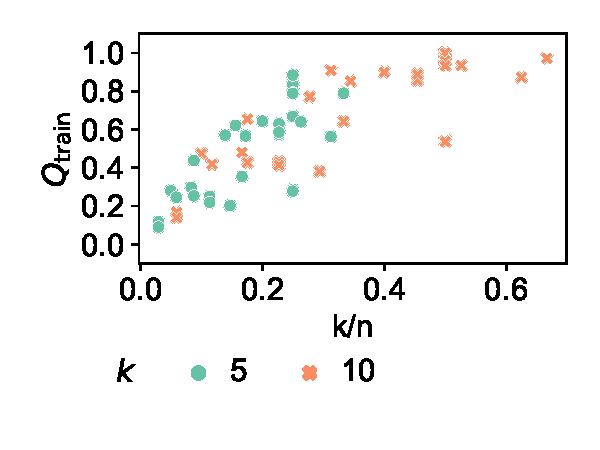
\includegraphics[width=\textwidth, trim=15 30 15 15, clip]{plots/impact-dataset-k-train-objective.pdf}
		\caption{Training-set objective value.}
		\label{fig:afs:impact-dataset-k-train-objective}
	\end{subfigure}
	\hfill
	\begin{subfigure}[t]{0.48\textwidth}
		\centering
		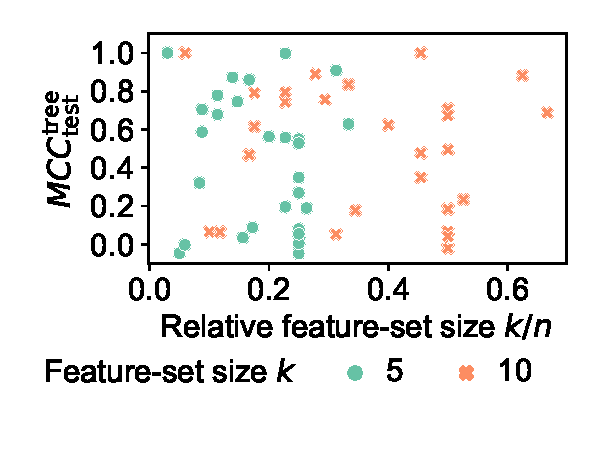
\includegraphics[width=\textwidth, trim=15 30 15 15, clip]{plots/impact-dataset-k-decision-tree-test-mcc.pdf}
		\caption{Test-set prediction performance for decision trees.}
		\label{fig:afs:impact-dataset-k-decision-tree-test-mcc}
	\end{subfigure}
	\caption{
		Quality of the original feature set over feature-set size~$k$ and datasets with sizes~$n$.
		Results from sequential search with \emph{MI} as feature selector.
	}
	\label{fig:afs:impact-dataset-k}
\end{figure}

Naturally, feature-set quality depends on the datasets used, and several effects could occur.
For example, the distribution of feature-set quality in the datasets might be relatively uniform or relatively skewed.
Datasets with more features $n$ give way to more alternative feature sets.
At the same time, the feature quality can be spread over more features than for smaller datasets, making it harder to compose a small high-quality feature set.

Indeed, our experiments show a broad variation of feature-set quality over the datasets.
Figure~\ref{fig:afs:impact-dataset-k} depicts the relationship between datasets and quality of the original feature set in sequential search.
To account for varying dataset size, we put the ratio between feature-set size~$k$ and dataset-size~$n$ on the x-axis, which is a measure of relative feature-set sizes.
As Figure~\ref{fig:afs:impact-dataset-k-train-objective} displays, the objective of an univariate feature selector approximately increases linearly with~$k/n$.
However, there still is some variation exclusively caused by the dataset rather than its dimensionality.
Further, the quality of a prediction model does not exhibit any trend but varies strongly between datasets, as Figure~\ref{fig:afs:impact-dataset-k-decision-tree-test-mcc} visualizes.
Due to this observed variation of feature-set quality between datasets, we normalize feature-set quality in some of the following analyses.

\subsection{Prediction Models}
\label{sec:afs:evaluation:prediction}

\begin{figure}[htb]
	\centering
	\begin{subfigure}[t]{0.48\textwidth}
		\centering
		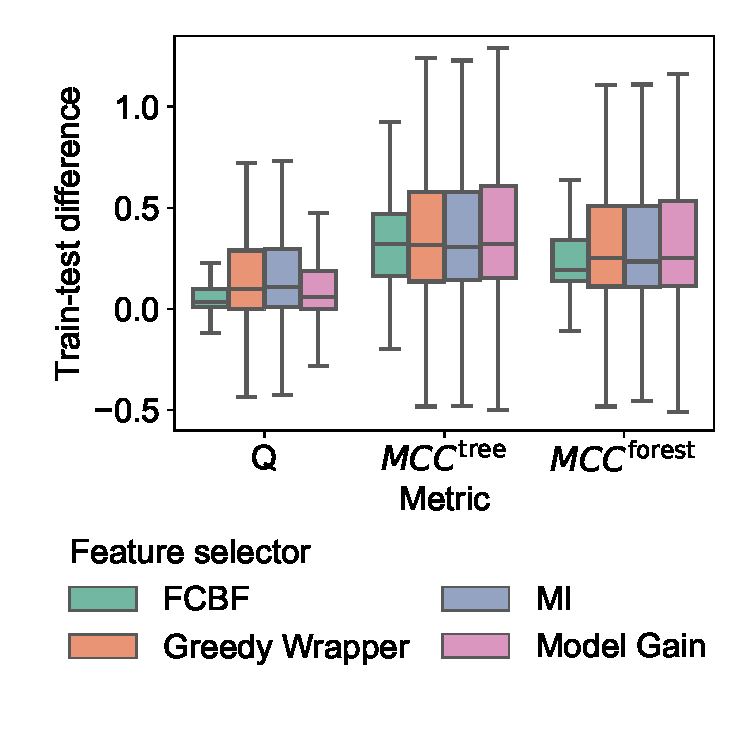
\includegraphics[width=\textwidth, trim=15 15 15 15, clip]{plots/evaluation-metrics-overfitting.pdf}
		\caption{
			Training-test difference over evaluation metrics and feature selectors.
			Outliers removed for readability reasons.
		}
		\label{fig:afs:evaluation-metrics-overfitting}
	\end{subfigure}
	\hfill
	\begin{subfigure}[t]{0.48\textwidth}
		\centering
		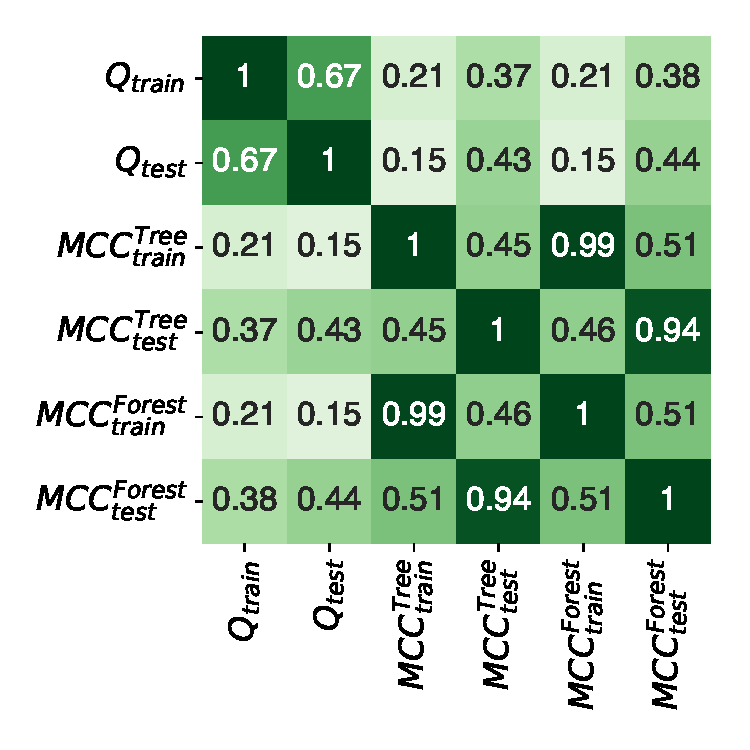
\includegraphics[width=\textwidth, trim=15 15 15 15, clip]{plots/evaluation-metrics-correlation.pdf}
		\caption{Correlation between the evaluation metrics calculated on the training set and the test set.}
		\label{fig:afs:evaluation-metrics-correlation}
	\end{subfigure}
	\caption{Comparison of evaluation metrics over all experimental settings.}
	\label{fig:afs:evaluation-metrics}
\end{figure}

As one can expect, the average prediction performance of random forests is higher than that of decision trees.
Also, overfitting occurs for both model types, i.e., there is a gap between training-set and test-set prediction performance.
In particular, over all experimental settings, decision trees and random forests both have a mean training-set MCC of 0.86 (median: 1.0).
In contrast, on the test set, decision trees have a mean MCC of 0.48 (median: 0.54), while random forests have a slightly higher mean MCC of 0.53 (median: 0.63).
Thus, average prediction performance is significantly worse on the test set than on the training set.
For a more detailed comparison, Figure~\ref{fig:afs:evaluation-metrics-overfitting} shows the distribution of the difference between training-set quality and test-set quality, again over all experimental settings.
Once more, we observe that training-set quality is usually higher, though there are a few cases where the difference becomes negative, i.e., test-set quality is higher.

The existence of overfitting makes sense as we do not regularize, i.e., limit the growth of, the trees or prune them after training.
However, this will not invalidate our analysis of how prediction performance develops over alternatives.
The optimization objective~$Q$, which Figure~\ref{fig:afs:evaluation-metrics-overfitting} also depicts, shows overfitting for all feature-selection methods as well, though to a lesser extent than for prediction performance.

Figure~\ref{fig:afs:evaluation-metrics-correlation} shows the Spearman correlation between different evaluation metrics.
As the performance of decision trees and random forests is highly correlated on training set as well as test set, we only focus on one prediction model in the following:
We choose decision trees, as they always consider all features during training, while random forests involve random sampling of features.

Figure~\ref{fig:afs:evaluation-metrics-correlation} also shows that the correlation between training-set quality and test-set quality is moderate, but not high, for the optimization objective~$Q$ as well as prediction performance in terms of MCC.
This might be caused by different degrees of overfitting, depending on the experimental settings.
Further, the correlation between optimization objective~$Q$ and prediction MCC is only weak to moderate.
I.e., the objective of feature selection is only partially indicative of prediction performance since the former might use a simplified quality criterion.

\subsection{Feature-Selection Methods}
\label{sec:afs:evaluation:feature-selection}

\begin{figure}[htb]
	\centering
	\begin{subfigure}[t]{0.48\textwidth}
		\centering
		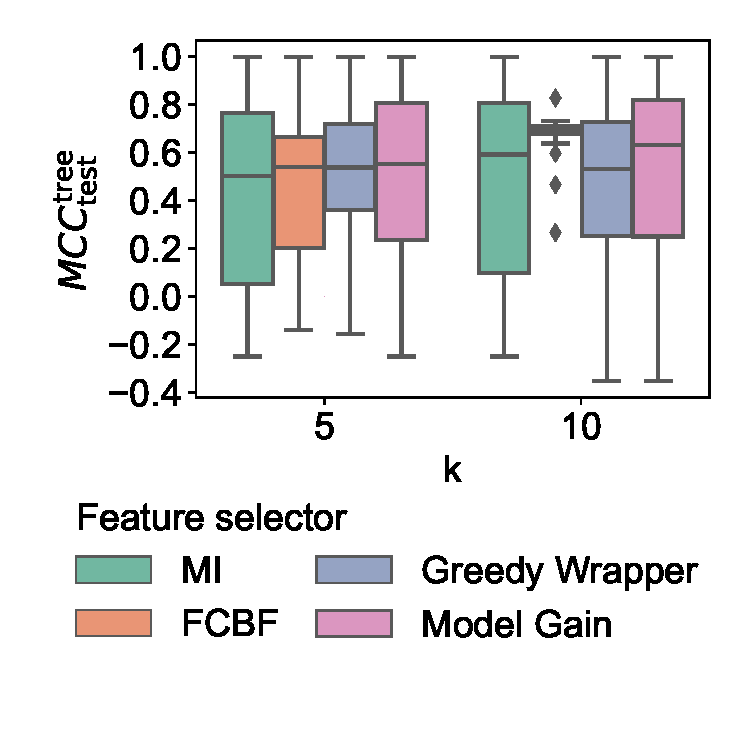
\includegraphics[width=\textwidth, trim=15 50 15 15, clip]{plots/impact-fs-method-k-decision-tree-test-mcc.pdf}
		\caption{Test-set prediction performance for decision trees.}
		\label{fig:afs:impact-fs-method-k-decision-tree-test-mcc}
	\end{subfigure}
	\hfill
	\begin{subfigure}[t]{0.48\textwidth}
		\centering
		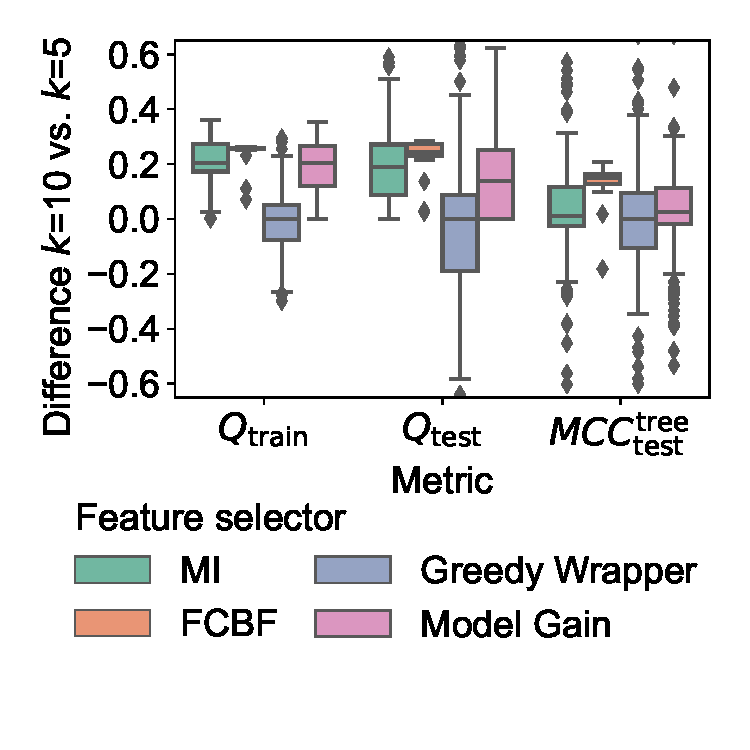
\includegraphics[width=\textwidth, trim=15 50 15 15, clip]{plots/impact-fs-method-k-metric-diff.pdf}
		\caption{
			Difference in feature-set quality between $k=10$ and $k=5$.
			Y-axis truncated for readability reasons.
		}
		\label{fig:afs:impact-fs-method-k-metric-diff}
	\end{subfigure}
	\caption{
		Comparison of feature selectors and feature-set sizes~$k$.
		Results from the original feature sets of sequential search.
	}
	\label{fig:afs:impact-fs-method-k}
\end{figure}

As the different feature-selection methods employ different objective functions~$Q$, it does not make sense to compare absolute objective values between feature-selection methods.
However, we can compare how useful the obtained feature sets are for predictions.
Figure~\ref{fig:afs:impact-fs-method-k-decision-tree-test-mcc} compares a decision tree's test-set prediction performance on the original feature sets of sequential search for different feature selectors.
On average, \emph{Model Gain} is the best feature selector, though not clearly better than the other selectors.
In particular, the median test-set MCC of decision trees is 0.59 for \emph{Model Gain}, 0.57 for \emph{FCBF}, and 0.54 for \emph{MI} and \emph{Greedy Wrapper}.
In particular, the univariate, model-free feature scoring with \emph{MI} keeps up surprisingly well with the more sophisticated methods.

The relatively bad performance of \emph{Greedy Wrapper} might result from its heuristic nature:
The wrapper search can only evaluate a fraction of all feasible feature sets and might get stuck in local optima, while the remaining feature-selection methods optimize globally.
In particular, \emph{Greedy Wrapper} only performed 63 iterations on average (median: 43) over all experimental settings.
Thus, it usually stayed significantly below the 1000~iterations we granted it.

Further, the results for \emph{FCBF} have to be taken with a grain of salt:
Over all experimental settings, 89\% of feature sets for \emph{FCBF} could not be determined, as the solver timed out or the optimization problem was infeasible.
In contrast, this figure only is 19\% for \emph{MI}.
Even the original feature set in sequential search is infeasible in 76\% of the cases for \emph{FCBF} but never for the other feature selectors.
In particular, the combination of feature-correlation constraints in our formulation of \emph{FCBF} (c.f.~Equation~\ref{eq:afs:fcbf}) with a feature-set-cardinality constraint seemingly made it hard to find valid feature sets.

As expected, larger feature sets, i.e., with~$k=10$, usually exhibit higher feature-set quality than smaller feature sets, i.e., $k=5$.
However, the increase in feature-set quality with $k$ is not proportional, and there might even be a decrease.
As Figure~\ref{fig:afs:impact-fs-method-k-metric-diff} shows for the original feature sets of sequential search, the exactly optimized feature selectors exhibit a slight increase of the training-set objective value~$Q_\mathrm{train}$ from~$k=5$ to~$k=10$.
As these objectives are monotonic in the feature selection, a decrease in quality is not possible.
In contrast, the heuristic \emph{Greedy Wrapper} does not necessarily benefit from selecting more features.
As Figure~\ref{fig:afs:impact-fs-method-k-metric-diff} also displays, the benefit of larger feature sets is even less clear for prediction performance, no matter which feature selector is used.
Thus, we will focus on smaller feature sets, i.e., $k=5$, in the following.

\subsection{Searching Alternatives}
\label{sec:afs:evaluation:search}

\subsubsection{Search Method}
\label{sec:afs:evaluation:search:method}

\begin{figure}[p]
	\centering
	\begin{subfigure}[t]{0.48\textwidth}
		\centering
		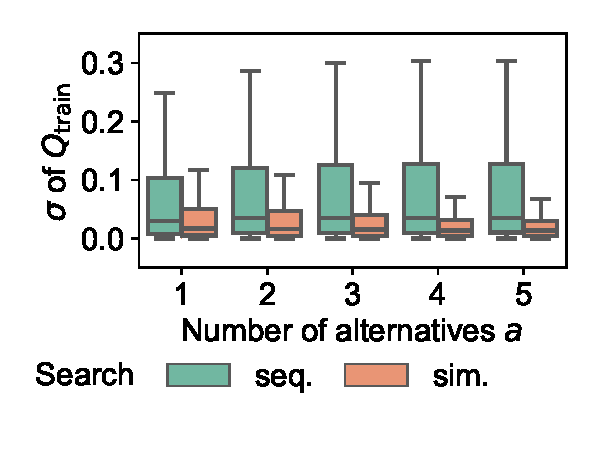
\includegraphics[width=\textwidth, trim=15 25 15 15, clip]{plots/impact-search-stddev-train-objective.pdf}
		\caption{Standard deviation of training-set objective value within individual search runs.}
		\label{fig:afs:impact-search-stddev-train-objective}
	\end{subfigure}
	\hfill
	\begin{subfigure}[t]{0.48\textwidth}
		\centering
		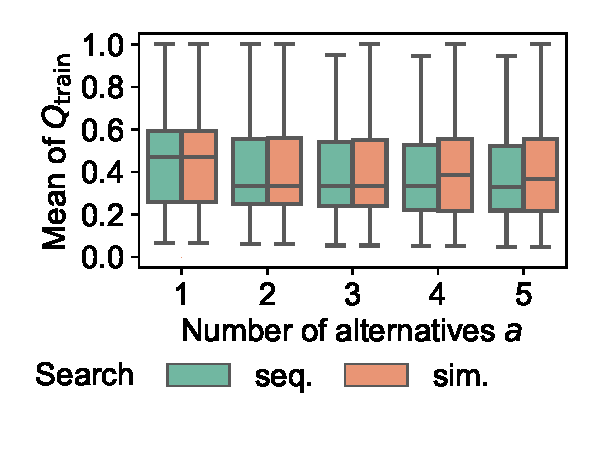
\includegraphics[width=\textwidth, trim=15 25 15 15, clip]{plots/impact-search-mean-train-objective.pdf}
		\caption{Mean of training-set objective value within individual search runs.}
		\label{fig:afs:impact-search-mean-train-objective}
	\end{subfigure}
	\\ \vspace{\baselineskip}
	\begin{subfigure}[t]{0.48\textwidth}
		\centering
		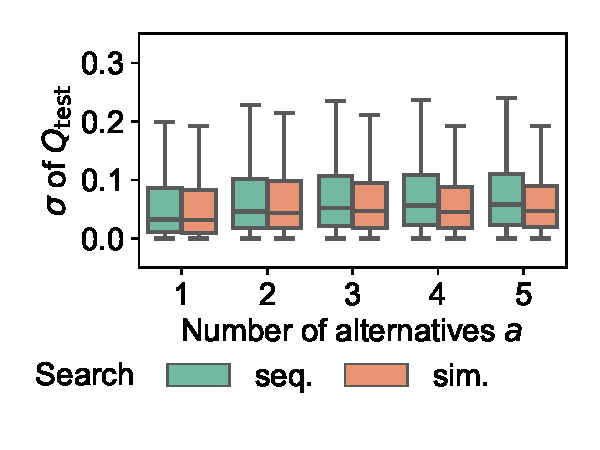
\includegraphics[width=\textwidth, trim=15 25 15 15, clip]{plots/impact-search-stddev-test-objective.pdf}
		\caption{Standard deviation of test-set objective value within individual search runs.}
		\label{fig:afs:impact-search-stddev-test-objective}
	\end{subfigure}
	\hfill
	\begin{subfigure}[t]{0.48\textwidth}
		\centering
		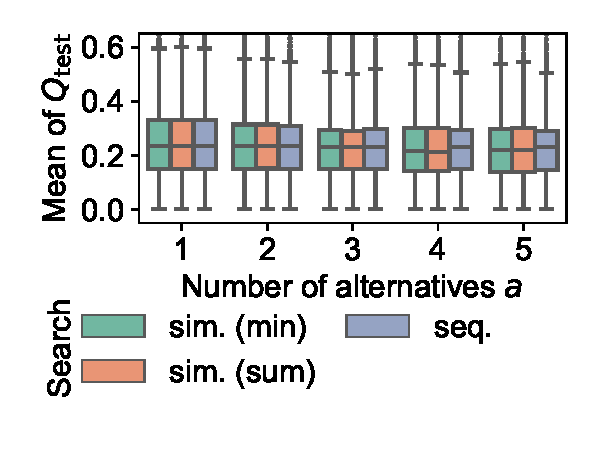
\includegraphics[width=\textwidth, trim=15 25 15 15, clip]{plots/impact-search-mean-test-objective.pdf}
		\caption{Mean of test-set objective value within individual search runs.}
		\label{fig:afs:impact-search-mean-test-objective}
	\end{subfigure}
	\\ \vspace{\baselineskip}
	\begin{subfigure}[t]{0.48\textwidth}
		\centering
		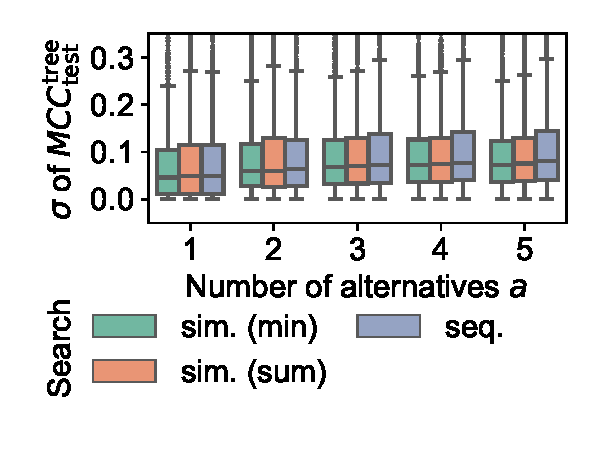
\includegraphics[width=\textwidth, trim=15 25 15 15, clip]{plots/impact-search-stddev-decision-tree-test-mcc.pdf}
		\caption{Standard deviation of test-set prediction performance for decision trees within individual search runs.}
		\label{fig:afs:impact-search-stddev-decision-tree-test-mcc}
	\end{subfigure}
	\hfill
	\begin{subfigure}[t]{0.48\textwidth}
		\centering
		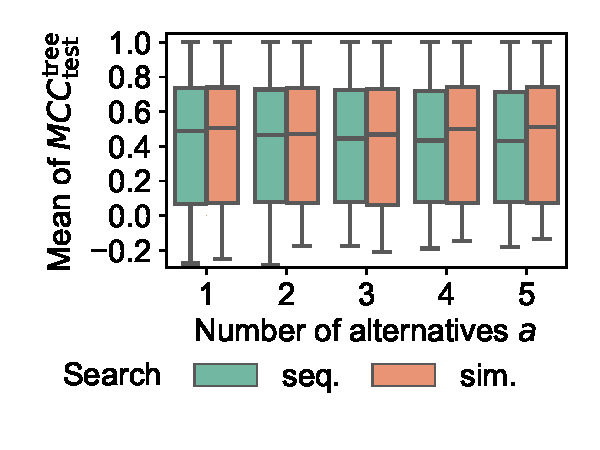
\includegraphics[width=\textwidth, trim=15 25 15 15, clip]{plots/impact-search-mean-decision-tree-test-mcc.pdf}
		\caption{Mean of test-set prediction performance for decision trees within individual search runs.}
		\label{fig:afs:impact-search-mean-decision-tree-test-mcc}
	\end{subfigure}

	\caption{
		Comparison of search methods for alternatives over the number of alternatives.
		Results with \emph{MI} as feature selector and $k=5$.
		Outliers removed for readability reasons.
	}
	\label{fig:afs:impact-search}
\end{figure}

\begin{figure}[htb]
	\centering
	\begin{subfigure}[t]{0.48\textwidth}
		\centering
		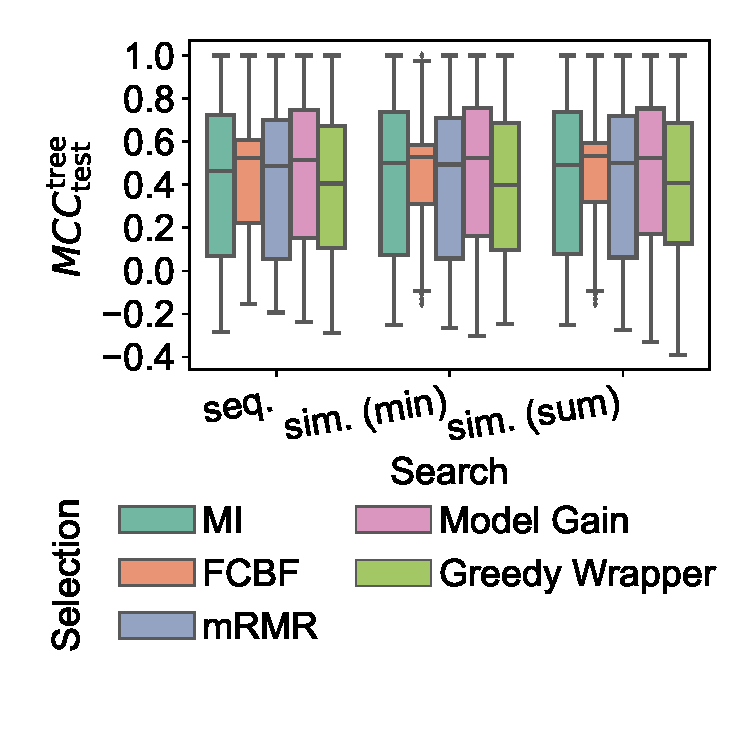
\includegraphics[width=\textwidth, trim=15 50 15 15, clip]{plots/impact-search-fs-method-decision-tree-test-mcc.pdf}
		\caption{Test-set prediction performance for decision trees.}
		\label{fig:afs:impact-search-fs-method-decision-tree-test-mcc}
	\end{subfigure}
	\hfill
	\begin{subfigure}[t]{0.48\textwidth}
		\centering
		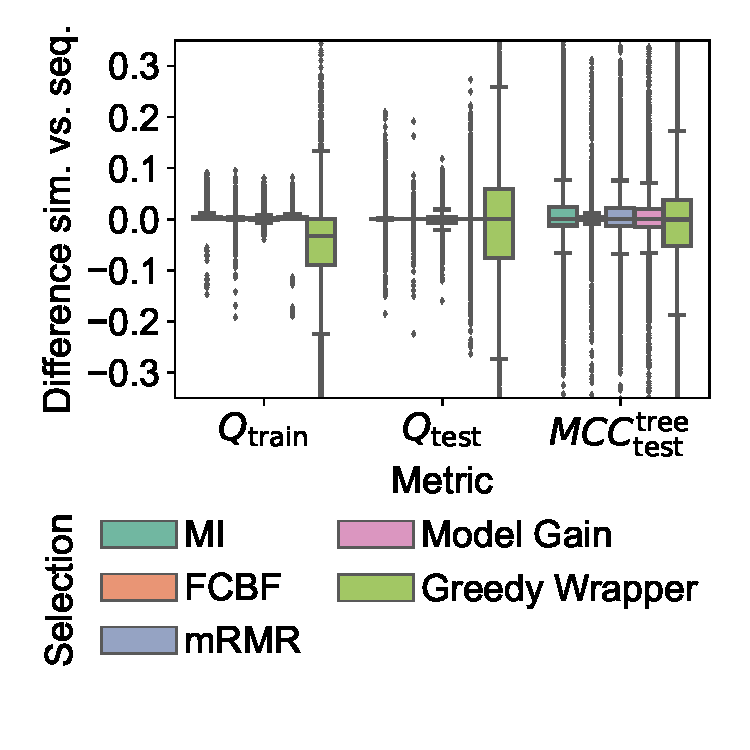
\includegraphics[width=\textwidth, trim=15 50 15 15, clip]{plots/impact-search-fs-method-metric-diff.pdf}
		\caption{
			Difference in feature-set quality between simultaneous and sequential search.
			Y-axis truncated for readability reasons.
		}
		\label{fig:afs:impact-search-fs-method-metric-diff}
	\end{subfigure}
	\caption{
		Comparison of feature selectors and search methods with $k=5$ and up to five alternatives.
	}
	\label{fig:afs:impact-search-fs-method}
\end{figure}

As we expected, the training-set objective value~$Q$ of feature sets within each particular search run usually varies more for sequential search than for simultaneous search.
I.e., simultaneous search tends to return alternatives with more homogeneous quality than sequential search.
Also, this variance decreases with the number of alternatives~$a$ for simultaneous search, but remains stable or slightly increases for sequential search.
Figure~\ref{fig:afs:impact-search-stddev-train-objective} visualizes these observations for \emph{MI} as feature selector and $k=5$.
These findings also apply to \emph{Model Gain} and partly to \emph{FCBF}, but not the heuristic \emph{Greedy Wrapper}.
We discuss the reasons for these inconsistencies later.
In contrast, using $k=10$ instead of $k=5$ does not change the general trends.

As Figure~\ref{fig:afs:impact-search-stddev-test-objective} shows, the difference in variance between sequential and simultaneous search is less prominent for the test-set objective value.
This effect might be a result of overfitting.
For the test-set prediction performance, visualized in Figure~\ref{fig:afs:impact-search-stddev-decision-tree-test-mcc}, the median variance within a search run differs even less between sequential and simultaneous search.
Thus, the actual prediction performance of multiple alternatives found by simultaneous search is not more homogeneous than for sequential search.

While obtaining alternatives of more homogeneous quality can be one goal of simultaneous search, the main selling point would be obtaining alternatives of higher average quality.
However, we found that simultaneous search is not clearly better than sequential search in that regard.
In particular, Figure~\ref{fig:afs:impact-search-mean-train-objective} compares the distribution of the mean training-set objective in search runs for \emph{MI} as feature selector and $k=5$.
We can see that simultaneous search only develops a slight comparative advantage against sequential search if the number of alternatives increases.
The same holds for \emph{Model Gain} as feature selector, while \emph{FBCF} does not show an advantage of simultaneous search on average and \emph{Greedy Wrapper} even tends to favor sequential search.

The negligible advantage of simultaneous search for \emph{MI} also is visible for the test-set prediction performance in Figure~\ref{fig:afs:impact-search-mean-decision-tree-test-mcc}.
In particular, as Figure~\ref{fig:afs:impact-search-fs-method-decision-tree-test-mcc} shows, other aspects than the search method, e.g., dataset, dissimilarity threshold~$tau$, etc. cause a significantly larger variation in prediction performance.
Further, regarding the test-set objective value, the median for simultaneous search even tends to become slightly worse than for sequential search, as Figure~\ref{fig:afs:impact-search-mean-test-objective}.

As a final comparison, Figure~\ref{fig:afs:impact-search-fs-method-metric-diff} displays the difference in evaluation metrics between the two search approaches if they are compared on each search setting separately, e.g., each dataset, fold, or dissimilarity threshold~$tau$.
The figure again shows that all feature selectors except \emph{Greedy Wrapper} exhibit little variation in quality between the two search approaches, apart from some outlying experimental settings.
Additionally, the figure highlights that outliers can occur in both directions:
While simultaneous search can yield better-performing feature sets in some situations, sequential search can be significantly better in other scenarios.

\begin{table}[htb]
	\centering
	\begin{tabular}{llrrrr}
		\toprule
		Selector & Search & \multicolumn{4}{c}{Optimization status} \\
		\cmidrule(r){3-6}
		& & Infeasible & Not solved & Feasible & Optimal \\
		\midrule
		FCBF & sequential & 70.25\% & 0.00\% & 0.00\% & 29.75\% \\
		FCBF & simultaneous & 67.47\% & 7.13\% & 5.01\% & 20.39\% \\
		MI & sequential & 1.97\% & 0.00\% & 0.00\% & 98.03\% \\
		MI & simultaneous & 4.67\% & 0.00\% & 8.49\% & 86.84\% \\
		Model Gain & sequential & 1.97\% & 0.00\% & 0.00\% & 98.03\% \\
		Model Gain & simultaneous & 4.67\% & 0.00\% & 7.16\% & 88.17\% \\
		\bottomrule
	\end{tabular}
	\caption{
		Frequency of optimization statuses by feature-selection method and search method with $k=5$ and up to five alternatives.
		Excluding \emph{Greddy Wrapper}, which calls the solver multiple times, and checks satisfiability rather than optimizing.
		Each row sums to 100\%.
	}
	\label{tab:afs:impact-search-fs-method-optimization-status}
\end{table}
%
\begin{table}[htb]
	\centering
	\begin{tabular}{rrrrr}
		\toprule
		$a$ & \multicolumn{4}{c}{Optimization status} \\
		\cmidrule(r){2-5}
		& Infeasible & Not solved & Feasible & Optimal \\
		\midrule
		1 & 21.33\% & 1.18\% & 0.00\% & 77.49\% \\
		2 & 21.73\% & 2.22\% & 0.02\% & 76.02\% \\
		3 & 23.96\% & 2.31\% & 1.07\% & 72.67\% \\
		4 & 29.96\% & 2.82\% & 3.04\% & 64.18\% \\
		5 & 31.02\% & 3.36\% & 30.31\% & 35.31\% \\
		\bottomrule
	\end{tabular}
	\caption{
		Frequency of optimization statuses by number of alternatives~$a$ in simultaneous search with $k=5$, excluding results from \emph{Greedy Wrapper} as feature selector.
		Each row sums to 100\%.
	}
	\label{tab:afs:impact-num-alternatives-optimization-status}
\end{table}
%
A major reason for simultaneous search not being advantageous is that results can be sub-optimal.
For \emph{Greedy Wrapper}, the search is heuristic per se, and only a tiny fraction of the search space is covered.
For the three exactly optimized feature-selection methods, the solver can time out.
As the optimization problem of simultaneous search is harder than for sequential search (cf.~Table~\ref{tab:afs:seq-sim-comparison}), it has a higher likelihood to run into timeouts.
Table~\ref{tab:afs:impact-search-fs-method-optimization-status} visualizes this phenomenon.
In particular, for up to five alternatives and $k=5$, all sequential searches for the three white-box feature selectors finished within the timeout, i.e., yielded the optimal feature set or ascertain infeasibility.
In contrast, 5.01\% of the simultaneous searches for \emph{FBCF}, 7.16\% for \emph{Model Gain} and 8.49\% for \emph{MI} found a feasible solution till the timeout but could not guarantee optimality.
Such a solution can be worse than an optimal sequential solutions.
Further, 7.13\% of the simultaneous searches for \emph{FBCF} found no feasible solution but could not guarantee infeasibility, i.e., a feasible solution might still exist.
Note that the fraction of timeouts strongly depends on the number of alternatives~$a$, as Table~\ref{tab:afs:impact-num-alternatives-optimization-status} displays:
For up to two alternatives in simultaneous search with $k=5$, barely any search runs yield feasible but potentially suboptimal results.
In contrast, this figure is roughly 1\% for three alternatives, 3\% for four alternatives and 30\% for five alternatives.

Based on all results described in this section, we focus on the sequential search in the following.
In particular, it appeared to be faster than simultaneous search while yielding similar feature-set quality.

\subsubsection{Number of Alternatives}
\label{sec:afs:evaluation:search:num-alternatives}

\begin{figure}[htbp]
	\centering
	\begin{subfigure}[t]{0.48\textwidth}
		\centering
		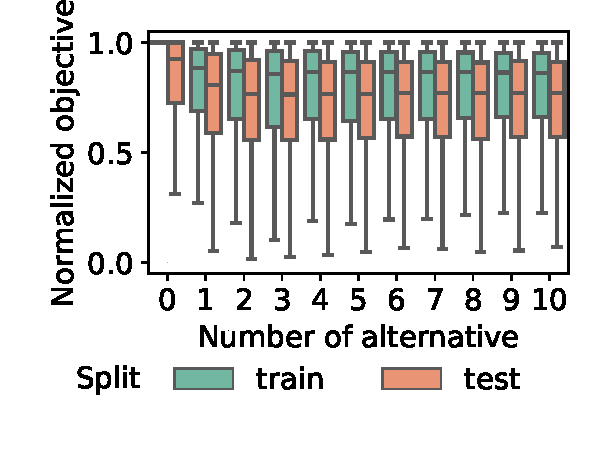
\includegraphics[width=\textwidth, trim=15 25 15 15, clip]{plots/impact-num-alternatives-objective-max.pdf}
		\caption{
			Objective value with max-normalization.
			Objective values of infeasible feature sets excluded.
		}
		\label{fig:afs:impact-num-alternatives-objective-max}
	\end{subfigure}
	\hfill
	\begin{subfigure}[t]{0.48\textwidth}
		\centering
		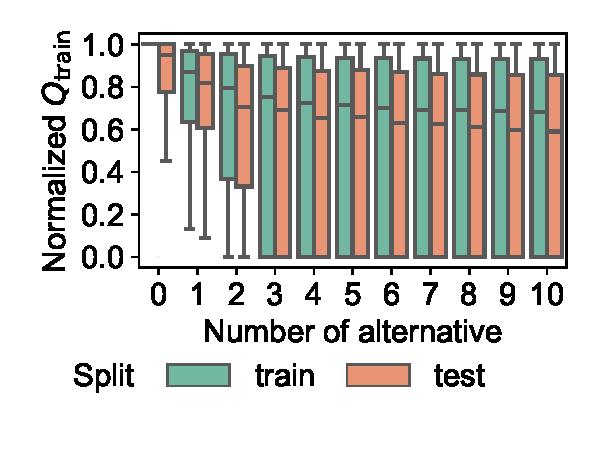
\includegraphics[width=\textwidth, trim=15 25 15 15, clip]{plots/impact-num-alternatives-objective-max-fillna.pdf}
		\caption{
			Objective value with max-normalization.
			Objective values of infeasible feature sets set to zero.
		}
		\label{fig:afs:impact-num-alternatives-objective-max-fillna}
	\end{subfigure}
	\\ \vspace{\baselineskip}
	\begin{subfigure}[t]{0.48\textwidth}
		\centering
		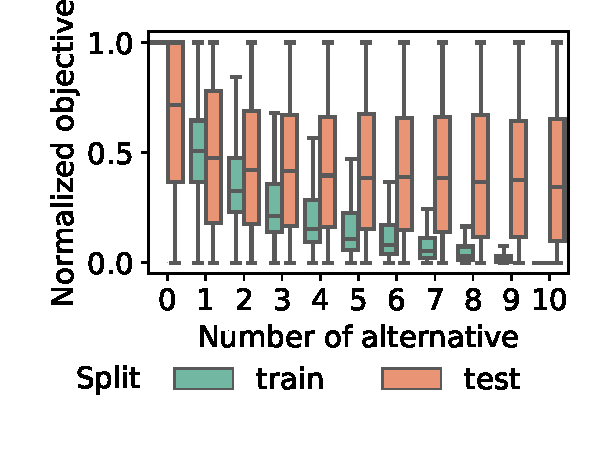
\includegraphics[width=\textwidth, trim=15 25 15 15, clip]{plots/impact-num-alternatives-objective-min-max.pdf}
		\caption{
			Objective value with min-max-normalization.
			Objective values of infeasible feature sets excluded.
		}
		\label{fig:afs:impact-num-alternatives-objective-min-max}
	\end{subfigure}
	\hfill
	\begin{subfigure}[t]{0.48\textwidth}
		\centering
		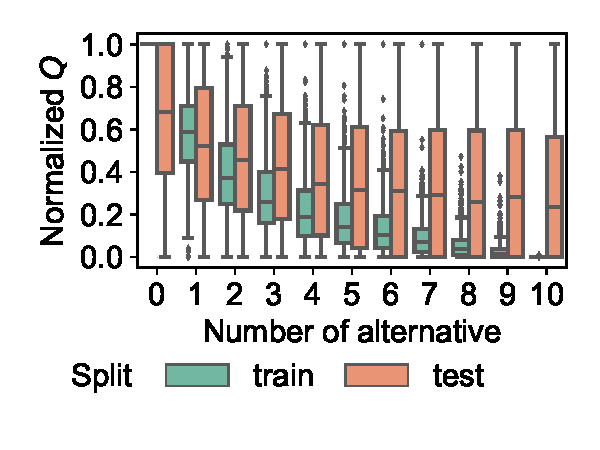
\includegraphics[width=\textwidth, trim=15 25 15 15, clip]{plots/impact-num-alternatives-objective-min-max-fillna.pdf}
		\caption{
			Objective value with min-max-normalization.
			Objective values of infeasible feature sets set to zero.
		}
		\label{fig:afs:impact-num-alternatives-objective-min-max-fillna}
	\end{subfigure}
	\\ \vspace{\baselineskip}
	\begin{subfigure}[t]{0.48\textwidth}
		\centering
		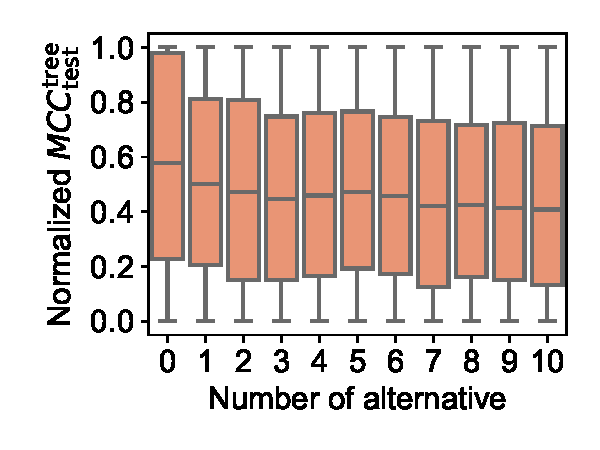
\includegraphics[width=\textwidth, trim=15 15 15 15, clip]{plots/impact-num-alternatives-decision-tree-test-mcc-min-max.pdf}
		\caption{
			Test-set prediction performance with min-max-normalization.
			Prediction performance of infeasible feature sets excluded.
		}
		\label{fig:afs:impact-num-alternatives-decision-tree-test-mcc-min-max}
	\end{subfigure}
	\hfill
	\begin{subfigure}[t]{0.48\textwidth}
		\centering
		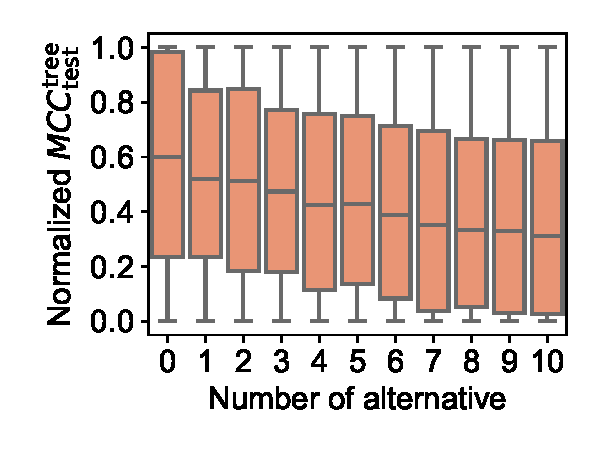
\includegraphics[width=\textwidth, trim=15 15 15 15, clip]{plots/impact-num-alternatives-decision-tree-test-mcc-min-max-fillna.pdf}
		\caption{
			Test-set prediction performance with min-max-normalization.
			Prediction performance of infeasible feature sets set to zero.
		}
		\label{fig:afs:impact-num-alternatives-decision-tree-test-mcc-min-max-fillna}
	\end{subfigure}

	\caption{
		Feature-set quality, normalized per experimental setting, over the number of alternatives.
		Results from sequential search with \emph{MI} as feature selector and $k=5$.
	}
	\label{fig:afs:impact-num-alternatives}
\end{figure}

For sequential search, the training-set objective value $Q$ naturally decreases with the number of alternatives, at least for the feature-selection criteria optimized exactly.
Figures~\ref{fig:afs:impact-num-alternatives-objective-max} and~\ref{fig:afs:impact-num-alternatives-objective-min-max} illustrate this for \emph{MI}-based feature selection.
The other feature-selection methods exhibit similar effects.
As feature-set quality varies between datasets, we apply normalization:
In Figure~\ref{fig:afs:impact-num-alternatives-objective-max}, we have max-normalized the objective value for each search of alternatives, i.e., the highest objective value in the search run is scaled to~1 and the other feature-set qualities are scaled accordingly.
This figure shows that there might be multiple alternatives of similar quality, as the median feature-set quality remains relatively stable over the number of alternatives, and is close to the maximum of~1.
For comparison, Figure~\ref{fig:afs:impact-num-alternatives-objective-min-max} uses min-max normalization, i.e., the worst of the alternatives gets~0 as objective.
This figure highlights that the training-set objective value decreases most from the original feature set to the first alternative but less beyond.

Additionally, Figures~\ref{fig:afs:impact-num-alternatives-objective-max} and~\ref{fig:afs:impact-num-alternatives-objective-min-max} show that the test-set objective value also drops most from the original feature set to the first alternative.
However, the decrease in objective value over the alternatives is less prominent than on the training set.
In particular, alternatives can even have a higher test-set objective value than the original feature set due to overfitting.
Similar findings hold for test-set prediction performance displayed in Figure~\ref{fig:afs:impact-num-alternatives-decision-tree-test-mcc-min-max}.
Thus, the alternative feature sets fulfill their purpose of being different solutions with similar quality.

Be aware that these observations refer to the quality of the found feature sets.
However, the more alternatives are desired, the more likely an infeasible optimization problem is.
For example, the \emph{MI} feature selector in sequential search always finds an original feature set.
However, with $k=5$, the problem is infeasible in 2\% of the cases for the third alternative, 12\% for the fifth alternative, and 18\% for the tenth alternative.
Increasing the feature-set size $k$, e.g., to $k=10$, or decreasing the dataset dimensionality~$n$, naturally increase the number of infeasibilities, as less features become available for alternatives.
Thus, while the quality of actually found feature sets seems to remain relatively stable with an increased number of alternatives, valid alternatives might simply not exist.
Figures~\ref{fig:afs:impact-num-alternatives-objective-max-fillna},~\ref{fig:afs:impact-num-alternatives-objective-min-max-fillna}, and~\ref{fig:afs:impact-num-alternatives-decision-tree-test-mcc-min-max-fillna} show the same data as Figures~\ref{fig:afs:impact-num-alternatives-objective-max},~\ref{fig:afs:impact-num-alternatives-objective-min-max}, and~\ref{fig:afs:impact-num-alternatives-decision-tree-test-mcc-min-max} but with the objective of infeasible feature sets set to zero.
This makes sense since selecting no features leads to such an objective value for \emph{MI}-based feature selection, and MCC is zero for randomly guessing predictions.
In these figures, the downward trend of feature-set quality over the number of alternatives becomes more prominent.
This trend also depends on the dissimilarity threshold $\tau$, which we analyze next.

\subsubsection{Dissimilarity Threshold \texorpdfstring{$\tau$}{}} % \texorpdfstring prevents warning "Token not allowed in a PDF string"
\label{sec:afs:evaluation:search:tau}

\begin{figure}[htb]
	\centering
	\begin{subfigure}[t]{0.48\textwidth}
		\centering
		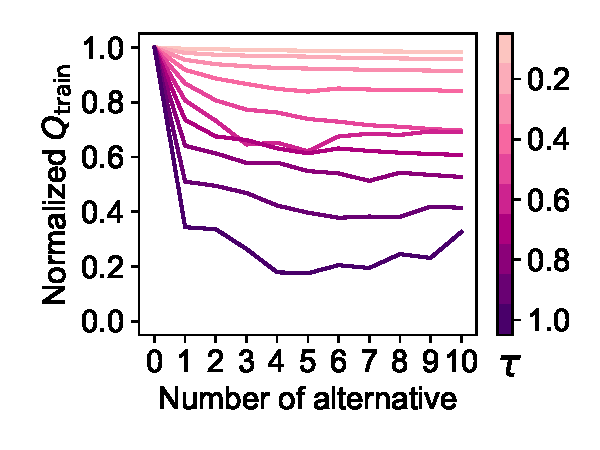
\includegraphics[width=\textwidth, trim=15 15 10 15, clip]{plots/impact-num-alternatives-train-objective-max-tau.pdf}
		\caption{Training set. Objective values of infeasible feature sets excluded.}
		\label{fig:afs:impact-num-alternatives-train-objective-max-tau}
	\end{subfigure}
	\hfill
	\begin{subfigure}[t]{0.48\textwidth}
		\centering
		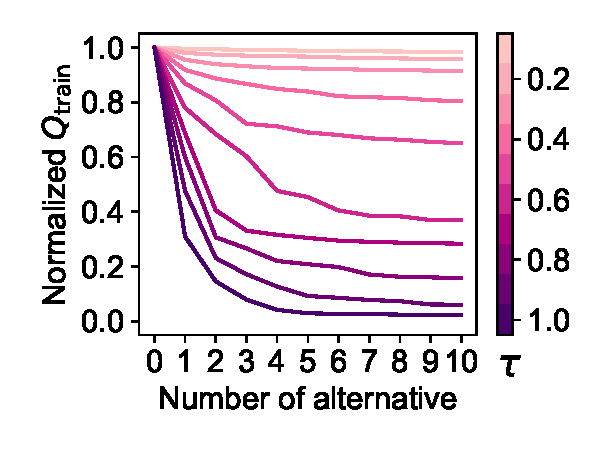
\includegraphics[width=\textwidth, trim=15 15 10 15, clip]{plots/impact-num-alternatives-train-objective-max-fillna-tau.pdf}
		\caption{Training set. Objective values of infeasible feature sets set to zero.}
		\label{fig:afs:impact-num-alternatives-train-objective-max-fillna-tau}
	\end{subfigure}
	\\ \vspace{\baselineskip}
	\begin{subfigure}[t]{0.48\textwidth}
		\centering
		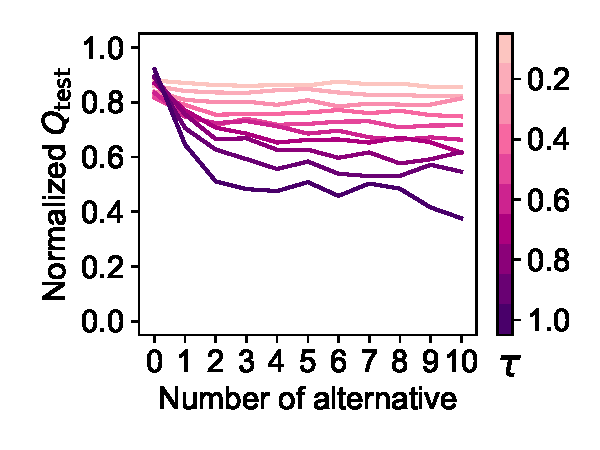
\includegraphics[width=\textwidth, trim=15 15 10 15, clip]{plots/impact-num-alternatives-test-objective-max-tau.pdf}
		\caption{Test set. Objective values of infeasible feature sets excluded.}
		\label{fig:afs:impact-num-alternatives-test-objective-max-tau}
	\end{subfigure}
	\hfill
	\begin{subfigure}[t]{0.48\textwidth}
		\centering
		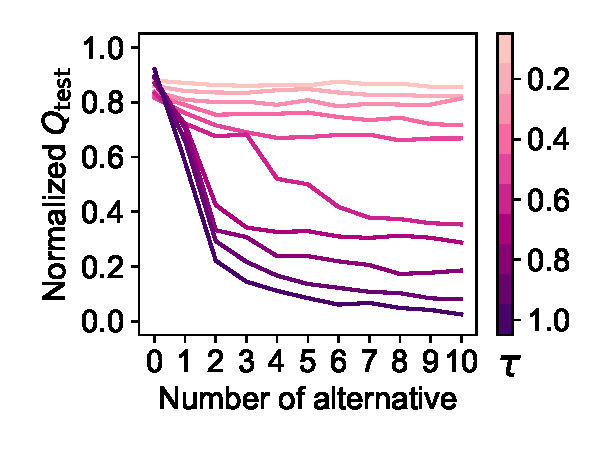
\includegraphics[width=\textwidth, trim=15 15 10 15, clip]{plots/impact-num-alternatives-test-objective-max-fillna-tau.pdf}
		\caption{Test set. Objective values of infeasible feature sets set to zero.}
		\label{fig:afs:impact-num-alternatives-test-objective-max-fillna-tau}
	\end{subfigure}
	\caption{
		Mean objective value $Q$, max-normalized per experimental setting, over the number of alternatives and dissimilarity threshold~$\tau$.
		Results from sequential search with \emph{MI} as feature selector and $k=10$.
		Outliers removed for readability reasons.
	}
	\label{fig:afs:impact-num-alternatives-objective-max-tau}
\end{figure}

As Figure~\ref{fig:afs:impact-num-alternatives-objective-max-tau} shows for \emph{MI} as feature selector, the decrease of the objective value $Q$ over the number of alternatives strongly depends on the dissimilarity threshold $\tau$.
For a low dissimilarity threshold, e.g., $\tau=0.1$, the objective value barely drops over the number of alternatives.
In contrast, the objective decrease significantly for a high dissimilarity threshold, e.g., $\tau=1$.
This phenomenon also holds for test-set objective and test-set prediction performance, though the decrease with $\tau$ is less prominent.
Also, the fraction of infeasible optimization problems, i.e., lack of valid alternative feature sets, increases with $\tau$:
For a higher dissimilarity threshold, the likelihood is higher that there is no feature set that is alternative enough.
Figures~\ref{fig:afs:impact-num-alternatives-train-objective-max-fillna-tau} and~\ref{fig:afs:impact-num-alternatives-test-objective-max-fillna-tau} demonstrate this by setting the objective value to zero if no feasible feature set could be found.
Compared to Figures~\ref{fig:afs:impact-num-alternatives-train-objective-max-tau} and~\ref{fig:afs:impact-num-alternatives-test-objective-max-tau}, the decrease in objective value is stronger.
In contrast, if only considering valid feature sets, the mean objective can increase over the number of alternatives, as visible in Figure~\ref{fig:afs:impact-num-alternatives-train-objective-max-tau} for $\tau=1.0$.
This is because some datasets run out of valid feature sets sooner than others, so the average quality is determined for different datasets at each number of alternatives.

While the previous observation were made for \emph{MI} as feature selector, they do not hold universally.
Besides \emph{MI}, the results for \emph{Model Gain} strongly depend on \emph{tau} as well.
In contrast, \emph{FCBF} and \emph{Greedy Wrapper} exhibit less influence of $\tau$ on feature-set quality.
For \emph{Greedy Wrapper}, this can be explained by its heuristic search procedure.
For \emph{FCBF}, the fraction of infeasible solutions is much higher than for \emph{MI} in general, so adding further constraints has less impact.

\section{Conclusions and Future Work}
\label{sec:afs:conclusion}

\subsection{Conclusions}

Obtaining interpretable solutions is a highly active research area in machine learning.
One way to foster interpretability is by selecting a small set of features for predictions.
Traditional feature-selection methods yield \emph{one} feature set with high quality, e.g., regarding prediction performance.
However, users might be interested in obtaining multiple, sufficiently different feature sets that, at the same time, have high quality.
Such alternative feature set might provide alternative explanations for predictions from the data.

In this paper, we defined alternative feature selection as an optimization problem.
We formalized alternatives via constraints, which are independent from the feature-selection method and can be combined with other constraints on feature sets, e.g., based on domain knowledge.
Further, we presented approaches to solve this optimization problem for different categories of feature selectors.
Finally, we ran an evaluation with 30 classification datasets and four feature-selection methods.
We compared two search strategies for alternatives and varied the threshold for being alternative.

In our experiments, we found that one can indeed obtain alternative feature sets with similar quality as the original ones, depending on the dataset and the parametrization for searching alternatives.
On average, simultaneous search and sequential search for alternatives yielded similar feature-set quality.
However, the latter procedure was significantly faster and generally allows stopping the search once the user does not want any more alternatives, so we recommend using it.
As expected, the quality of alternatives dropped the more alternatives one desired, and the more alternatives should differ from existing feature sets.
The ultimate decision on which trade-off between feature-set quality and alternatives is acceptable lies with the user.
Thus, we recommend evaluating different dissimilarity thresholds for alternatives to find a suitable value.

\subsection{Future Work}

While our work introduced alternative feature selection, there are several points for applying, extending, or modifying the latter.

\paragraph{Feature selection (objective function)}

One can search for alternatives with other feature-selection methods than the four we analyzed.
For wrapper feature selection, which requires black-box optimization, there are multiple ways to consider alternatives (cf.~Section~\ref{sec:afs:approach:objectives:black-box}).
As we saw in our experiments, achieving a high feature-set quality within a reasonable time frame poses a particular challenge for this category of feature-selection methods.
Further, our generic search procedures need adaptation to work for the category of embedded feature selection (cf.~Section~\ref{sec:afs:approach:objectives:embedding}), which we did not consider in our experiments.

\paragraph{Alternatives (constraints)}

One can vary the notion of alternatives (cf.~Sections~\ref{sec:afs:approach:problem} and~\ref{sec:afs:approach:constraints}), e.g., the set-dissimilarity measure, the definitions for multiple alternatives, or by using soft constraints instead of hard constraints.
While we tried to make general and straightforward decisions for each of these points, particular applications might demand other formal definitions of alternatives.

\paragraph{Simultaneous alternatives}

Our experiments (cf.~Section~\ref{sec:afs:evaluation:search:method}) as well as theoretical analysis (cf.~Section~\ref{sec:afs:approach:constraints:multiple}) revealed that simultaneous search scales badly with the number of alternatives.
One way to alleviate this is finding a more efficient problem formulation, e.g., by loosening the constraints for alternatives.
However, looser constraints bear the danger of allowing identical feature sets as valid alternatives.
Further, one can limit the solver runtime and take the intermediate results once the timeout is reached.
We already used a fixed timeout in our experiments, but studying the exact impact of different timeouts one the feature-set quality is a topic for future work.
Finally, one can use a different solver, e.g., one that supports non-linear terms so the interaction variables and constraints from Equation~\ref{eq:afs:product-linear} become superfluous.

\paragraph{Datasets}

Our evaluation builds on benchmark datasets from various domains.
While we could uncover several general trends, the existence and the quality of alternative feature sets clearly depends on the dataset (cf.~Section~\ref{sec:afs:evaluation:datasets}).
Thus, practitioners can use our generic approaches to search alternatives in domain-specific case studies.

\appendix

\section{Appendix}
\label{sec:afs:appendix}

\subsection{Min-Quality Objective for Simultaneous Alternatives}
\label{sec:afs:appendix:min-quality-objective}

In this section, we present another objective for simultaneous search.
In Equation~\ref{eq:afs:afs-simultaneous}, we use the summed feature-set quality over alternatives as the objective.
While this objective fosters a high average quality of feature sets, it does not guarantee that the alternatives have similar quality, though the latter could be a goal for searching simultaneously.
For example, consider univariate filter feature selection (cf.~Equation~\ref{eq:afs:univariate-filter}) with five features, the feature qualities~$q = (1,2,3,4,5)$, desired feature-set size $k=2$, and dissimilarity threshold $\tau = 1$, i.e., allowing no overlap of feature sets.
The feature selection $s^{(0)} = (0,0,0,1,1)$, $s^{(1)} = (0,1,1,0,0)$ yields the optimal summed quality of $9+5=14$, while the quality of these two feature sets differs significantly.
The feature selection $s^{(0)} = (0,1,0,0,1)$, $s^{(1)} = (0,0,1,1,0)$ yields the same summed quality of $7+7=14$ but with balanced feature-set qualities.
Sequential search for alternatives can only yield the first, quality-imbalanced solution due to the greedy search procedure.
Simultaneous search with the summed-quality objective could yield both solutions, due to the identical objective value, so we still cannot be sure to get balanced qualities.

To actively foster balanced feature-set qualities in simultaneous search, we can use the minimum instead of the sum over $Q(\cdot)$ in the objective:
%
\begin{equation}
	\begin{aligned}[t]
		&\quad \max_{s^{(0)}, \dots, s^{(a)}} & \min_{i \in \{0, \dots, a\}} Q(s^{(i)},X,y) \\
		\text{instead of:} &\quad \max_{s^{(0)}, \dots, s^{(a)}} & \sum_{i=0}^a Q(s^{(i)},X,y)
	\end{aligned}
	\label{eq:afs:afs-simultaneous-min-objective}
\end{equation}
%
In the terms of social choice theory, this re-formulated objective uses an egalitarian rule instead of a utilitarian one~\cite{myerson1981utilitarianism}.
As a downside, the summed feature-set quality can decrease under this new objective.
Also, we have no control or guarantee how much the feature-set qualities will actually differ since we only incentive high quality for all feature sets.
As another problem formulation, one could add constraints that limit the difference between the feature sets' qualities.
However, this formulation would introduce a new parameter for the allowed quality difference.
Alternatively, one could explicitly constrain the minimum or maximum quality of all feature sets, which also introduces one or several parameters that are difficult to determine a priori.
Instead of using further constraints, one could consider balanced feature sets' qualities as another objective besides the maximizing the summed quality, but then the user would have to handle an implicit trade-off between the objectives.

From the technical perspective, Equation~\ref{eq:afs:afs-simultaneous-min-objective} has the disadvantage of being a non-linear expression regarding the decision variables $s^{(0)}, \dots, s^{(a)}$.
However, we can linearize it with the help of an auxiliary variable~$Q_{\text{min}}$ and one additional constraint per feature set:
%
\begin{equation}
	\begin{aligned}
		\max_{s^{(0)}, \dots, s^{(a)}} &\quad &Q_{\text{min}} & \\
		\text{subject to:} &\quad \forall i \in \{0, \dots, a\} : &Q_{\text{min}} &\leq Q(s^{(i)},X,y) \\
		&\quad & Q_{\text{min}} &\in \mathbb{R}
	\end{aligned}
	\label{eq:afs:afs-simultaneous-min-objective-linear}
\end{equation}
%
As we maximize~$Q_{\text{min}}$, this variable will implicitly assume the actual minimum value of~$Q(s^{(i)},X,y)$ with equality since the solution would not be optimal otherwise.
This situation relives us from introducing further auxiliary variables that are usually necessary when linearizing maximum or minimum expressions~\cite{mosek2022modeling}.

\subsection{Complete Specifications of the Optimization Problem}
\label{sec:afs:appendix:complete-optimization-problem}

In this section, we provide complete specifications of the alternative-feature-selection problem for sequential and simultaneous search.
In particular, we combine all relevant definitions and equations from Section~\ref{sec:afs:approach}.
For the objective, we consider an univariate filter feature selector, as defined in the Equation~\ref{eq:afs:univariate-filter}.
The corresponding feature qualities $q(\cdot)$ are constants in the optimization problem.
To measure feature-set dissimilarity for alternatives, we use the Dice dissimilarity from Equation~\ref{eq:afs:dice-rearranged-equal-size}.
The dissimilarity threshold~$\tau \in [0,1]$ is a user-defined constant.
Further, we assume that each feature set should have a fixed, user-defined size~$k \in \mathbb{N}$, as in our experiments.

\paragraph{Sequential alternatives}

In the sequential case, only one feature set~$F_s$ is variable.
In contrast, the existing feature sets $F_{\bar{s}} \in \mathbb{F}$ with their selection vectors $\bar{s}$ are constants in the optimization problem.
%
\begin{equation}
	\begin{aligned}
		\max_s &\quad & Q_{\text{uni}}(s,X,y) &= \sum_{j=1}^{n} q(X_{\cdot{}j},y) \cdot s_j \\
		\text{subject to:} &\quad \forall F_{\bar{s}} \in \mathbb{F} :& \sum_{j=1}^n s_j \cdot \bar{s}_j &\leq (1 - \tau) \cdot k \\
		&\quad & \sum_{j=1}^n s_j &= k \\
		&\quad & s &\in \{0,1\}^n
	\end{aligned}
	\label{eq:afs:afs-sequential-complete}
\end{equation}
%
\paragraph{Simultaneous alternatives}

In the simultaneous case, all feature sets are variable.
Let~$a \in \mathbb{N}$ denote the number of alternatives, which corresponds to the number of feature sets minus one.
Further, we introduce auxiliary variables according to Equation~\ref{eq:afs:product-linear} to linearize products between variables.
%
\begin{equation}
	\begin{aligned}
		\max_{s^{(0)}, \dots, s^{(a)}} &\quad & \sum_i Q_{\text{uni}}(s^{(i)},X,y) &= \sum_i \sum_j q(X_{\cdot{}j},y) \cdot s^{(i)}_j\\
		\text{subject to:} &\quad \forall i_1~\forall i_2 :& \sum_j t^{(i_1,i_2)}_j &\leq (1 - \tau) \cdot k \\
		&\quad \forall i_1~\forall i_2~\forall j :& t^{(i_1,i_2)}_j &\leq s^{(i_1)}_j \\
		&\quad \forall i_1~\forall i_2~\forall j :& t^{(i_1,i_2)}_j &\leq s^{(i_2)}_j \\
		&\quad \forall i_1~\forall i_2~\forall j :& 1 + t^{(i_1,i_2)}_j &\geq s^{(i_1)}_j + s^{(i_2)}_j \\
		&\quad \forall i :& \sum_j s^{(i)}_j &= k \\
		&\quad \forall i :& s^{(i)} &\in \{0,1\}^n \\
		&\quad \forall i_1~\forall i_2 :& t^{(i_1,i_2)} &\in \{0,1\}^n \\
		\text{with indices:} &\quad & i,~i_1 &\in \{0, \dots, a\} \\
		&\quad & i_2 &\in \{0, \dots, i_1-1\} \\
		&\quad & j &\in \{1, \dots, n\}
	\end{aligned}
	\label{eq:afs:afs-simultaneous-complete}
\end{equation}

\subsection{Finding Alternatives for Univariate Feature Qualities}
\label{sec:afs:appendix:univariate-search-algorithm}

For an objective consisting of univariate feature qualities (cf.~Equation~\ref{eq:afs:univariate-filter} and Section~\ref{sec:afs:appendix:complete-optimization-problem}), one can easily find a limited number of optimal alternative feature sets without a solver.
To this end, we propose the following \emph{greedy-replacement} procedure, displayed in Algorithm~\ref{al:afs:greedy-replacement}:

The univariate objective function does not contain interaction terms between features.
Thus, we start by sorting the features decreasingly according to their individual qualities~$q_j$.
Given a desired feature-set size~$k$, the optimal original feature set, i.e., the zeroth alternative, simply consists of the first~$k$ features from this quality-based ordering.
Depending on the set-dissimilarity measure defining alternatives, one can then determine how many features needs to differ for obtaining a valid alternative.
For the Dice dissimilarity we use in our paper, including Algorithm~\ref{al:afs:greedy-replacement}, $\lceil \tau \cdot k \rceil$~features need to differ between feature sets (cf.~Equation~\ref{eq:afs:dice-rearranged-equal-size}).
Consequently, a fixed subset of $\lfloor (1 - \tau) \cdot k \rfloor$~features can be contained in all alternatives without violating the dissimilarity threshold.
Thus, for each alternative, we always select the best $\lfloor (1 - \tau) \cdot k \rfloor$~features regarding quality~$q_j$.
We only replace the remaining $\lceil \tau \cdot k \rceil$~features from alternative to alternative.
To this end, we fill up the feature sets with the highest-quality features that were not part of any feature set yet, which ensures a sufficient pairwise dissimilarity between feature sets.
We continue this procedure till we reach the desired number of alternatives or till there are not enough unused features to form further alternatives.

\begin{algorithm}[htb]
	\DontPrintSemicolon
	\KwIn{Univariate feature qualities~$q_j$ with $j \in \{1, \dots, n\}$, \newline
		Feature-set size~$k$, \newline
		Number of alternatives~$a$, \newline
		Dissimilarity threshold~$\tau$}
	\KwOut{Feature-selection decision vectors~$s^{(\cdot)}$}
	\BlankLine
	\If(\tcp*[f]{Not enough features for selection}){$k > n$}{
		\Return{$\emptyset$}
	}
	$indices \leftarrow$ sort\_indices($q$, order=descending) \tcp*{Order by qualities}
	$s \leftarrow \{0\}^n$ \tcp*{Initial selection for all alternatives}
	$position \leftarrow 1$ \tcp*{Index of index of currently selected feature}
	\While{$position < \lfloor (1 - \tau) \cdot k \rfloor$}{
		$j \leftarrow indices[position]$\;
		$s_j \leftarrow 1$ \;
		$position \leftarrow position + 1$\;
	}
	$i \leftarrow 0$\ \tcp*{Number of current alternative}
	\While{$i \leq a$ \textbf{and} $i \leq \frac{n - k}{\lceil \tau \cdot k \rceil}$}{
		$s^{(i)} \leftarrow s$ \tcp*{Select best $\lfloor (1 - \tau) \cdot k \rfloor$ features}
		\For(\tcp*[f]{Select remaining $\lceil \tau \cdot k \rceil$ features}){$\_ \leftarrow 1$ \KwTo $\lceil \tau \cdot k \rceil$}{
			$j \leftarrow indices[position]$\;
			$s^{(i)}_j \leftarrow 1$\;
			$position \leftarrow position + 1$\;
		}
		$i \leftarrow i + 1$\;
	}
	\Return{$s^{(0)}, \dots, s^{(i)}$}
	\caption{Greedy-replacement search for alternative feature sets based on Dice dissimilarity.}
	\label{al:afs:greedy-replacement}
\end{algorithm}

For example, with $n=10$ features, feature-set size~$k=5$, and $\tau=0.4$, each feature set has to differ by two features from the other feature sets.
The original feature set consists of the five best features regarding quality~$q(\cdot)$.
The first alternative consists of the three best features plus the sixth- and seventh-best feature.
The second alternative consists of the three best features plus the eight- and ninth-best feature.
After that alternative, the greedy-replacement procedure has to stop, as there are not enough unused features to form further alternatives.
In general, the $\lfloor (1 - \tau) \cdot k \rfloor$~best features plus the $k + (i-1) \cdot \lceil \tau \cdot k \rceil + 1$ to $k + i \cdot \lceil \tau \cdot k \rceil$~best features form the $i$-th alternative.

One can also adapt this procedure to permit varying feature-set sizes~$k^{(i)}$ over alternatives rather than using a constant~$k$.
Especially, if one knows the values of all~$k^{(i)}$ beforehand, one can still compute the admissible overlap of feature sets (cf. Equation~\ref{eq:afs:dice-rearranged}) and thereby determine the number of features to be replaced per iteration.
However, if the order of the $k^{(i)}$-values is flexible, the situation becomes more involved.
In particular, assembling feature sets of different sizes in different order can result in a different overall objective value, i.e., summed feature-set quality.

In contrast, for a fixed~$k$, not even a simultaneous search can surpass the summed quality of the solutions yielded by the sequential greedy-replacement procedure, though the former might compose the feature sets differently.
However, greedy replacement only works as long as some features have not been part of any feature set yet, i.e., $k + i \cdot \lceil \tau \cdot k \rceil \leq n$.
Once this pool of unused features is exhausted, one would need another strategy to find further alternatives.
Additionally, continuing search from the results of greedy replacement might then perform worse than a simultaneous search.
Thus, to obtain a high number of alternatives with greedy replacement, the following conditions are beneficial:
The number of features~$n$ should be high, the feature-set size~$k$ show be low, and the dissimilarity threshold~$\tau$ should be low.
These conditions align well with classical feature-selection scenarios where~$k \ll n$.

Besides the drawback of potentially running out of unused features, there are further disadvantages of greedy replacement compared to solver-based optimization.
In particular, greedy replacement does not work once the optimization problem gets more involved.
For example, there might be further constraints on feature sets, e.g,, based on domain knowledge, which are not accounted for in Algorithm~\ref{al:afs:greedy-replacement}.
Also, the objective function becomes more complex for other feature selectors than univariate filters, which makes the quality-based feature ordering impossible or suboptimal.
At most, one could start with the original feature set from a sophisticated feature selector and then continue with greedy replacement based on univariate qualities.
Simultaneous search with the min-quality objective from Appendix~\ref{sec:afs:appendix:min-quality-objective} also is unsuitable for greedy replacement.
Overall, greedy replacement is a fast search procedure for special scenarios, but a solver-based search for alternatives is more general.
Our experiments in Section~\ref{sec:afs:evaluation} consistently use a solver.

\subsection{Objectives for Multivariate Filter Feature Selectors}
\label{sec:afs:appendix:multivariate-filter-objectives}

While Section~\ref{sec:afs:approach:objectives:white-box} already addressed FCBF, we discuss the objective functions for CFS~\cite{hall1999correlation, hall2000correlation}, mRMR~\cite{peng2005feature}, and Relief~\cite{kira1992feature, robnik1997adaptation} here.

\paragraph{CFS}

Correlation-based Feature Selection (CFS)~\cite{hall1999correlation, hall2000correlation} considers both relevance and redundancy of features.
Relevance is the correlation between features and prediction target, similar to the univariate filter.
Redundancy is the correlation between features, acting as a normalization term.
Using a bivariate dependency measure $q$ to quantify correlation, the objective is as follows:
%
\begin{equation}
	Q_{\text{CFS}}(s,X,y) = \frac{\sum_{j=1}^{n} q(X_{\cdot{}j},y) \cdot s_j}{\sqrt{\sum_{j=1}^{n} s_j + \sum_{j_1=1}^{n} \sum_{\substack{j_2=1 \\ j_2 \neq j_1}}^{n} q(X_{\cdot{}j_1}, X_{\cdot{}j_2}) \cdot s_{j_1} \cdot s_{j_2}}}
	\label{eq:afs:cfs}
\end{equation}
%
One can also square this objective to get rid off the square root in the denominator~\cite{nguyen2010towards}.
Nevertheless, the objective is non-linear in the decision variables~$s$ since it involves a fraction and multiplications between variables.
However, one can linearize the objective with additional variables and constraints~\cite{nguyen2010improving, nguyen2010towards}.

\paragraph{mRMR}

Minimal Redundancy Maximum Relevance (mRMR)~\cite{peng2005feature} follows a similar principle as CFS, but uses the difference instead of the ratio between a relevance term and a redundancy term:
%
\begin{equation}
	Q_{\text{mRMR}}(s,X,y) = \frac{\sum_{j=1}^{n} q(X_{\cdot{}j},y) \cdot s_j}{\sum_{j=1}^{n} s_j} - \frac{\sum_{j_1=1}^{n} \sum_{j_2=1}^{n} q(X_{\cdot{}j_1}, X_{\cdot{}j_2}) \cdot s_{j_1} \cdot s_{j_2}}{(\sum_{j=1}^{n} s_j)^2}
	\label{eq:afs:mrmr}
\end{equation}
%
If one knows the feature-set size, the denominators are constant and thus, Equation~\ref{eq:afs:mrmr} is linear if one replaces the product terms with Equation~\ref{eq:afs:product-linear}.
Without this replacement, the objective leads to a quadratic-programming problem~\cite{nguyen2014effective, rodriguez2010quadratic}, though there is a linearization as well~\cite{nguyen2009optimizing, nguyen2010towards}.

\paragraph{Relief}

Relief~\cite{kira1992feature, robnik1997adaptation} assigns a score to each feature by sampling data objects and considering the difference in feature values compared to their nearest neighbors.
The idea is that data objects with a similar value of the prediction target should have similar feature values.
In contrast, data objects that differ in their prediction target should differ in their feature values as well.
We consider Relief to be multivariate as the nearest-neighbor computations involve all features instead of considering features independently.
However, the resulting scores for each feature can directly be put into the univariate-filter objective from Equation~\ref{eq:afs:univariate-filter}.
Further, one can use Relief scores in CFS to consider feature redundancy~\cite{hall1999correlation, hall2000correlation}, which the default Relief does not.

\renewcommand*{\bibfont}{\small} % use a smaller font for bib than for main text
\printbibliography

\end{document}
